\documentclass[12pt, a4paper]{report}

\usepackage[utf8]{inputenc}
\usepackage{graphicx}
\usepackage{times}

\usepackage{geometry}
\geometry{
    margin=1.2in,
    bottom=1.0in,
    headheight=8pt,
    headsep=0.2in,
    footskip=0.6in
}

\usepackage{setspace}
\onehalfspacing

\usepackage{tocloft}
\usepackage{fancyhdr}
\usepackage{tabularx}
\usepackage{enumitem}
\usepackage[table]{xcolor}
\usepackage{float}
\usepackage[section]{placeins}

\usepackage{tikz}
\usetikzlibrary{shapes.geometric, positioning, arrows.meta}

\graphicspath{{./images/}{./chapters/chapter3/images/}}

\usepackage{adjustbox}
\usepackage[hidelinks]{hyperref}
\usepackage{caption}
\captionsetup[table]{skip=6pt}
\usepackage{enumitem}
\usepackage{url}
\usepackage{hyperref}
\setcounter{tocdepth}{3}
\setcounter{secnumdepth}{3}


\pagestyle{fancy}
\fancyhf{}
\renewcommand{\headrulewidth}{0pt}
\renewcommand{\footrulewidth}{1pt}

\fancyfoot[L]{Digital Admission Procedure Management for Post-GST Candidates}
\fancyfoot[R]{Page | \thepage}

\fancypagestyle{plain}{
  \fancyhf{}
  \fancyfoot[L]{Digital Admission Procedure Management for Post-GST Candidates}
  \fancyfoot[R]{Page | \thepage}
  \renewcommand{\headrulewidth}{0pt}
  \renewcommand{\footrulewidth}{1pt}
}

\renewcommand{\contentsname}{Table of Contents}

\begin{document}

\pagenumbering{roman}

\begin{titlepage}
\begin{center}

\vspace*{0.5cm}

% Title
{\huge \textbf{JUST Undergraduate Final Admission System} \par}

\vspace{1.2cm}

% Subtitle
{\large \textbf{A Project Report Submitted} \par}
\vspace{0.2cm}
{\normalsize In partial fulfillment of the requirements for the degree of \par}
\vspace{0.1cm}
{\normalsize \textbf{B.Sc. Engineering in Computer Science and Engineering} \par}

\vspace{0.8cm}

% Logo

\includegraphics[width=0.22\textwidth]{images/images.jpeg}

\vspace{0.8cm}

% Student Info
{\large \textbf{Submitted by} \par}
\vspace{0.2cm}
{\normalsize \textbf{Nafis Ahamed} \par}
{\normalsize Student ID: 200129 \par}
{\normalsize Session: 2020--21 \par}

\vfill

% Supervisor
{\large \textbf{Supervised by} \par}
\vspace{0.2cm}
{\normalsize \textbf{Dr. Mohammad Nowsin Amin Sheikh} \par}
{\normalsize Assistant Professor \par}

\vspace{0.8cm}

% University Info
{\normalsize Department of Computer Science and Engineering \par}
{\normalsize Faculty of Engineering and Technology \par}
{\normalsize Jashore University of Science and Technology \par}
{\normalsize Jashore-7408, Bangladesh \par}

\vspace{0.4cm}

{\normalsize \textbf{April 2026} \par}

\end{center}
\end{titlepage}
\newpage
\sloppy   

\begin{center}
    \textbf{\large CERTIFICATE}
\end{center}

\vspace{0.8cm}

\noindent
This project titled, \textbf{Digital Admission Procedure Management for Post-GST Candidates}, developed by \textbf{Nafis Ahamed (Student ID: 200129)} has been accepted as satisfactory in partial fulfillment of the requirements for the degree {B.Sc (Engg.) in Computer Science and Engineering} in April 2026.

\vspace{2cm}

\noindent
\begin{minipage}[t]{0.55\textwidth}
    \textbf{Supervisor} \\[1.5cm]
    \rule{7cm}{0.5pt} \\
    {Dr. Mohammad Nowsin Amin Sheikh} \\
    Associate Professor \\
    Department of CSE \\
    Jashore University of Science and Technology \\
    Jashore-7408, Bangladesh
\end{minipage}
\hfill
\begin{minipage}[t]{0.4\textwidth}
    \raggedleft
    \textbf{Submitted by} \\[1.5cm]
    \rule{6cm}{0.5pt} \\
    {Nafis Ahamed} \\
    Student ID: 200129 \\
    Session: 2020--21
\end{minipage}

\vspace{3cm}

\begin{center}
\begin{minipage}[t]{0.75\textwidth}
    \centering
    \textbf{Chairman} \\[1.5cm]
    \rule{8cm}{0.5pt} \\
    {Md. Kamrul Islam} \\
    Assistant Professor \\
    Department of Computer Science and Engineering \\
    Jashore University of Science and Technology \\
    Jashore-7408, Bangladesh
\end{minipage}
\end{center}

\newpage
\begin{center}
    \Large \textbf{ACKNOWLEDGEMENT}
\end{center}

\vspace{1cm}

\noindent I want to say thank you to God, who helped me finish this work.

\vspace{0.5cm}

\noindent I am thankful to my project supervisor \textbf{Dr.Mohammad Nowsin Amin Sheikh}, Assistant Professor, Department of Computer Science and Engineering Jashore University of Science and Technology for helping me all the time. He gave me ideas and supported me a lot during this project.

\vspace{0.5cm}

\noindent I also want to thank the Chairman of our department \textbf{Md.Kamrul Islam}, Associate Professor for giving me advice and encouraging me from start to finish.

\vspace{0.5cm}

\noindent The project was successful because of Computer Science and Engineering project and the people who helped me.

\vspace{0.5cm}

\noindent I am really grateful, to my parents, who always supported me and helped me finish this work. They gave me everything I needed and motivated me to keep going. My parents are the reason I was able to finish this work. I thank them for that.

\vspace{2cm}

\noindent
\begin{minipage}[t]{0.4\textwidth}
    \rule{5cm}{0.4pt} \\
    {Nafis Ahamed} \\
    Student ID: 200129
\end{minipage}
\include{abstract}
\newpage
\begin{center}
    \Large \textbf{Preface}
\end{center}

\vspace{0.7cm}

\noindent On the eve of the beginning of civilization, human beings had been striving tirelessly to discover, explore, and innovate unknown aspects of the world. This inherent curiosity and desire for advancement have driven humanity toward continuous progress and development. Over time, human beings have not only acquired theoretical knowledge but have also emphasized the importance of practical implementation, which plays a crucial role in solving real-world problems and improving the quality of life.

\vspace{0.5cm}

\noindent In the modern era, the field of Computer Science and Engineering has emerged as one of the most dynamic and influential disciplines, contributing significantly to technological advancement and digital transformation. The philosophy of the Computer Science and Engineering department is centered on equipping students with both theoretical understanding and practical skills. To achieve this goal, the department has introduced thesis and project programs that encourage students to engage in real-life problem-solving and innovative system development.

\vspace{0.5cm}

\noindent As a part of fulfilling the academic requirements of the undergraduate program, I have undertaken a project titled \textbf{JUST Undergraduate Final Admission System}. This project aims to develop a comprehensive web-based platform that simplifies and streamlines the admission process for undergraduate students. It focuses on efficiency, transparency, and user-friendliness, ensuring a better experience for both applicants and administrators.

\vspace{0.5cm}

\noindent Throughout the development of this project, I have conducted extensive research, analysis, and observation to understand the existing admission processes and identify their limitations. This has enabled me to design and implement a system that addresses real-world challenges effectively. The project has provided me with valuable opportunities to enhance my technical skills, problem-solving abilities, and understanding of software development methodologies.

\vspace{0.5cm}

\noindent I believe that this project will not only serve as an academic accomplishment but also contribute positively to the automation and digitalization of admission systems. The knowledge and experience gained during this work will undoubtedly play a vital role in my future career and professional development.


\newpage
\tableofcontents

\newpage
\listoftables
\listoffigures

\newpage
\newpage
\section*{List of Abbreviations}

\vspace{0.5cm}

\begin{table}[H]
\renewcommand{\arraystretch}{1.5} 
\begin{tabular}{|l|p{10cm}|} 
\hline
\textbf{JUST} & Jashore University of Science and Technology \\ \hline
\textbf{DAPM-PGC} & Digital Admission Procedure Management for Post-GST Candidates \\ \hline
\textbf{CSE} & Computer Science and Engineering \\ \hline
\textbf{SRS} & Software Requirement Specification \\ \hline
\textbf{GST} & General, Science and Technology \\ \hline
\textbf{ERD} & Entity Relationship Diagram \\ \hline
\textbf{UI} & User Interface \\ \hline
\textbf{UX} & User Experience \\ \hline
\textbf{API} & Application Programming Interface \\ \hline
\textbf{SQL} & Structured Query Language \\ \hline
\textbf{RDBMS} & Relational Database Management System \\ \hline
\textbf{SDLC} & Software Development Life Cycle \\ \hline
\textbf{MVC} & Model-View-Controller \\ \hline
\textbf{JSON} & JavaScript Object Notation \\ \hline
\textbf{IEEE} & Institute of Electrical and Electronics Engineers \\ \hline
\end{tabular}
\end{table}

\newpage
\pagenumbering{arabic}
\pagestyle{fancy}

\chapter{Introduction}


\section{Chapter Overview}
The chapter highlights a brief discussion about the problem statement and the rationale behind undertaking this project. It starts by providing a brief introduction to the university admission process concerning the post-GST university admission process, wherein there are several stages of verification necessary to accomplish the entire process of admission. The rationale behind this project is based on the current state of affairs regarding the process of university admission. Presently, the admission process is carried out either manually or semi-manually, leading to inefficiencies in data management, which can be erroneous and slow, and poor communication between students and various departments within the university.Finally, the chapter states the objectives of the project.

\section{Background}

\noindent Admission of a university is an indispensable activity in every educational activity and is as old as education itself. With more students applying for admission than in previous years, admission process for admissions officers has become increasingly time-consuming. More applications resulted in heavier paperwork and processing challenges. Every admission is routed through various faculty for evaluation, and the manual admission process caused difficulty in admission, and archiving. 

\vspace{0.3cm}

\noindent In order to speed up and simplify the admission process, the development of the Automated Final Admission System is to enact document redesign and an automated management program. The proposed ``Digital Admission Procedure Management for Post-GST Candidates'' would store, route, and retrieve prospective and current application documents. The development of science and technology has immensely contributed to the growth of computers and the internet which has adversely increased the use and need for an automated applicant's admission system. 

\vspace{0.3cm}

\noindent Universities, Colleges, Companies, organizations, etc. are seeking better ways to distribute and disseminate information throughout the world. In order to achieve this, they develop and rely on online applications, which help them input, update, process, and disseminate information. The internet has increased the use of online applications because data could be easily and readily accessed as well as documented. This project is targeted at allowing admission of applicants' decisions to be made faster and more efficiently. It looks at improving the present traditional system of the manual process (paper-based) which is manually documented. This type of project is a hot topic in the whole world to digitalize our education system.
\section{Motivation}

\subsection{Existing System}
\noindent There are several automated systems used for managing final admission processes in educational institutions. These systems differ in features, capabilities, and implementation depending on institutional needs and available resources.

\vspace{0.3cm}

\noindent Currently, JUST provides a web-based application titled ``JUST Admission 2025''. While this system includes some useful functionalities, it is not a fully integrated or complete solution. Several important features are missing, such as admission confirmation, sending admission confirmation messages, and verification of required documents.

\vspace{0.3cm}

\noindent Another issue in the current system is that any user can register regardless of whether they have been selected for admission or not. This creates inconsistency and reduces system reliability. Additionally, the system lacks proper validation mechanisms, which makes it difficult to ensure the authenticity and correctness of submitted data.

\vspace{0.3cm}

\subsection{Limitations of the System}
\noindent The current system suffers from several limitations that affect its efficiency and usability.

\vspace{0.3cm}

\noindent First, there is no proper validation process implemented. As a result, users can input incorrect or incomplete data without restriction. Second, the system allows unrestricted data insertion but does not provide proper mechanisms for updating or removing data, which can lead to data inconsistency.

\vspace{0.3cm}

\noindent Third, the system architecture and code structure are not well organized, making it difficult to maintain, scale, or extend the system in the future.

\vspace{0.3cm}

\noindent Another significant limitation is that users who are not eligible (i.e., those who did not get a chance for admission) can still register in the system. This reduces the accuracy and trustworthiness of the admission process.

\vspace{0.3cm}

\noindent Finally, key features such as admission confirmation, automated message sending, and document verification are either missing or not fully implemented, which prevents the system from functioning as a complete automated admission solution.
\clearpage
\section{Objectives}

The main goal of this project is to create a web-based admission system that's easy to use and works well. This system will help with the following:

\begin{itemize}

    \item {Efficiency:} We want to make the admission process automatic to save time and make it easier to handle data. The system will help reduce work.

    \item {Accuracy:} We aim to reduce mistakes by minimizing data entry. This will ensure that application data and documents are handled correctly.

    \item {Consistency:} The system will process all data and applications in the way. This will reduce the risk of data and data loss.

    \item {Validation and Reliability:} We will put in place checks to ensure only eligible candidates can register. The system will also ensure that candidates submit information.

    \item {Performance:} We will use modern technologies to make the system work better and more reliably.

    \item {Security:} We will update the systems security measures to protect user data. This will prevent people from accessing the system without permission.

    \item {Scalability:} The software will be designed in such a way that it is scalable and will have an adaptive nature to accommodate more and more users and applications. It will also allow for future additions like features, departments, and even admissions.

\item {Usability:} The system will provide ease of use for students, staff members, and other users to perform their tasks smoothly without any complications.

\item {Maintainability:} The software will be designed with a well-defined architecture that can make it easy to update, maintain, and enhance in the future.

\item {Transparency:} The system will provide transparency in the process of admission. Users will always be able to see how far their admission applications have progressed.

\end{itemize}

\clearpage


\newpage
\section{Preface}

\subsection{Contributors}
The project titled \textbf{Digital Admission Procedure Management for Post-GST Candidates} was completed by \textbf{Nafis Ahamed (Student ID: 200129)} in partial fulfillment of the requirements for the degree of Bachelor of Science in Computer Science and Engineering. This work was accomplished under the constant guidance and valuable supervision of \textbf{Dr. Mohammad Nowsin Amin Sheikh}, Associate Professor, Department of Computer Science and Engineering at Jashore University of Science and Technology. His continuous feedback, constructive criticisms, and insightful suggestions played a vital role in refining the project and ensuring the quality of the final product.

\subsection{Chapter Organization}
The current report is organized into six chapters to present all aspects of the project systematically:

\begin{itemize}[leftmargin=1.5cm]
    \item \textbf{Chapter 1: Introduction} – Provides the foundational information, including the background, motivation, and objectives behind the development of the system.
    \item \textbf{Chapter 2: Software Requirement Specification} – Details the SRS, covering the system overview, user classes, constraints, and both functional and non-functional requirements.
    \item \textbf{Chapter 3: Design and Methodology} – Explains the program design, methodology applied, use-case diagrams, and the database schema.
    \item \textbf{Chapter 4: Implementation} – Focuses on the technical implementation of the program and the description of various modules.
    \item \textbf{Chapter 5: Testing} – Discusses the testing strategies and quality assurance measures taken to ensure system reliability.
    \item \textbf{Chapter 6: Deployment} – Covers the final deployment process and future scope of the project.
\end{itemize}

% \newpage
\chapter{\mbox{Software Requirement Specification}}
\label{ch:srs}

% To remove indentation for the entire chapter
\setlength{\parindent}{0pt}
% To add space between paragraphs since indent is 0
\setlength{\parskip}{1em} 

\section{Introduction}

\subsection{Purpose}

The main goal of the Undergraduate Final Admission System (JUST-DAPM-PGC) is to give a safe, fast and easy-to-use platform for finishing the final admission process. The old manual and semi-automated system had problems, including no checks, bad code, no structured design, and no way to enforce deadlines. This system is the fully integrated solution made by the JUST Undergraduate Admission Committee, aiming to fix existing problems by adding checks, controlling deadlines, giving different access levels to users, and offering a more scalable design.

This Software Requirement Specification (SRS) document explains the workflow of the final admission process, which includes applicants filling out forms, the Dean Office clearing applicants with required documents, the Hall Office verifying bank receipts, the Medical Center doing exams and reporting results, the Registrar Office giving approval and collecting documents, and administrative control for managing users, roles, and system operations.

\subsection{Document Conventions}

The following conventions are used in this SRS document:

\begin{itemize}
    \item Section headings are numbered.
    \item \textbf{Bold text} shows terms or concepts.
    \item All figures and tables have labels and numbers.
    \item The following abbreviations are used:
    \begin{itemize}
        \item JUST: Jashore University of Science and Technology.
        \item SRS: Software Requirements Specification.
        \item DAPM-PGC: Digital Admission Procedure Management for Post-GST Candidates.
    \end{itemize}
\end{itemize}

\subsection{Intended Audience and Reading Suggestions}

This document follows IEEE SRS standards. It is for the Admission Committee members, Project Supervisor, Chairman of the CSE Department, Internal and External Viva Board Members, future developers and system maintainers, and any stakeholders interested in understanding the Undergraduate Final Admission System (JUST-DAPM-PGC). Readers should start with the Introduction and Overall Description sections before moving to requirements.
\section{Overall Description}

\subsection{Product Perspective}
The JUST-DAPM-PGC is a web-based automated admission management system designed to replace the existing manual and partially digital processes. The previous system lacked critical features such as proper validation mechanisms, deadline enforcement, and structured system architecture.

\medskip
\noindent The proposed system introduces:
\begin{itemize}[leftmargin=1.5cm, labelsep=0.5cm]
    \item Strong input validation to prevent invalid or incomplete submissions.
    \item Deadline control to restrict registration and updates after the admission deadline.
    \item Role-based access control to ensure secure and authorized operations.
    \item A modular and maintainable architecture following modern design patterns.
    \item Real-time tracking of application progress across different offices.
    \item Scalability to handle a large number of concurrent applicants.
\end{itemize}

\subsection{Product Functions}
The major functionalities of the JUST-DAPM-PGC are as follows:

\begin{itemize}[leftmargin=0.5cm]
    \item[] Admin Module: 
    This module takes care of administration activities such as assigning different roles to users and setting the system security features. Administrators can keep track of the status of the admissions process through the use of this module.
    \begin{itemize}
        \item Manage users and roles.
        \item Control system operations (open/close admission).
        \item Monitor overall admission progress.
    \end{itemize}
    
    \vspace{0.2cm}
    \item[] Dean Office Module: 
    Charged with the responsibility of evaluating the academic qualifications of students through verification of education certificates. The Dean’s office makes it possible to either approve or disapprove applications depending on individual faculty requirements.
    \begin{itemize}
        \item Verify documents and validate applicants.
        \item Approve or reject applications.
        \item Export applicant data.
    \end{itemize}
    
    \vspace{0.2cm}
    \item[] Hall Office Module: 
    Deals with all financial and residence related issues such as the clearance of payment of admission costs using bank slips. This module ensures that all required residence clearance activities are completed for students requiring on-campus accommodation.
    \begin{itemize}
        \item Verify bank receipts.
        \item Manage residential clearance.
    \end{itemize}
    
    \vspace{0.2cm}
    \item[] Medical Center Module: 
    Enables the health evaluation process by capturing applicant’s medical details and carrying out physical examinations. This module creates medical reports which provide required health clearance before completing the admissions process.
    \begin{itemize}
        \item Record medical data.
        \item Generate reports and provide clearance.
    \end{itemize}
    
    \vspace{0.2cm}
    \item[] Registrar Office Module: 
    The last resort in the approval of applications for admissions. The module collects, stores and manages the information of admitted students through archiving of documents.
    \begin{itemize}
        \item Final admission approval.
        \item Document collection and archiving.
    \end{itemize}
    
    \vspace{0.2cm}
    \item[] Applicant Module: 
    The module helps the students register themselves, update their profile information, and apply for admissions by submitting the application form. The applicant can upload all relevant documents and even download important cards/notifications.
    \begin{itemize}
        \item Registration and profile management.
        \item Application form submission.
        \item Document upload and download.
    \end{itemize}
\end{itemize}
\section{User Classes and Characteristics}

The system includes multiple user roles, each with specific responsibilities. All users are expected to have basic knowledge of computers and web browsers.

\textbf{Admin:}
\begin{itemize}
    \item Full system control.
    \item Manage users and roles.
    \item Control admission deadlines.
\end{itemize}

\textbf{Dean Office:}
\begin{itemize}
    \item Verify documents.
    \item Approve or reject applications.
\end{itemize}

\textbf{Hall Office:}
\begin{itemize}
    \item Verify payment and clearance.
\end{itemize}

\textbf{Medical Office:}
\begin{itemize}
    \item Generate medical reports.
\end{itemize}

\textbf{Registrar Office:}
\begin{itemize}
    \item Final admission approval.
\end{itemize}

\textbf{Applicant:}
\begin{itemize}
    \item Submit application.
    \item Upload documents.
    \item Track status.
\end{itemize}
\section{Constraints}

The system operates under the following constraints:
\begin{itemize}
    \item Admission is strictly controlled by deadlines.
    \item No registration or updates allowed after deadline.
    \item All inputs must pass validation rules.
    \item Role-based access control is enforced.
    \item Requires stable internet connection.
    \item Security measures must protect user data.
\end{itemize}
\section{External Interface Requirements}

\subsection{User Interfaces}
The system provides a web-based user interface designed for simplicity and usability. Interfaces are role-based, ensuring that each user (Admin, Dean Office, Hall Office, Medical Office, Registrar Office, Applicant) can only access permitted features.

The interface includes:
\begin{itemize}
    \item Clear navigation and dashboard
    \item Form validation with proper instructions
    \item Role-specific panels for efficient task completion
\end{itemize}

\subsection{Integration with Existing Data}
The system supports integration with pre-existing admission data provided by the administration in Excel format. The admin uploads this data, which is then used to generate applicant accounts.

\subsection{Integration with Internal Modules}
All modules (Dean, Hall, Medical, Registrar) are interconnected and share a centralized database to ensure real-time updates and consistency.

\subsection{Authentication and Authorization}
The system implements secure authentication and role-based authorization:
\begin{itemize}
    \item Admin provides login credentials to users
    \item Applicants log in using GST Application ID
    \item Access control ensures users can only perform authorized actions
\end{itemize}

% System Features Sections
\section{System Features: Admin Management}

\subsection{Description and Priority}
The Admin module has the highest priority and controls the entire system. The admin uploads applicant data (Excel file), manages users, controls admission deadlines, and monitors all activities.

\subsection{Functional Requirements}

\textbf{Authentication}
\begin{itemize}
    \item Input: Username and password
    \item Output: Secure login access
\end{itemize}

\textbf{Upload Applicant Data}
\begin{itemize}
    \item Input: Excel file containing applicant information
    \item Output: System generates applicant accounts
\end{itemize}

\textbf{Manage Users}
\begin{itemize}
    \item View, update, and delete users
\end{itemize}

\textbf{Update Applicant Information}
\begin{itemize}
    \item Modify applicant data if required
\end{itemize}

\textbf{Control Admission}
\begin{itemize}
    \item Open or close admission system
\end{itemize}

\textbf{View Reports}
\begin{itemize}
    \item Monitor admission progress and seat status
\end{itemize}
\section{System Features: Dean Office}

\subsection{Description}
The Dean Office verifies applicant information and approves or rejects applications based on eligibility criteria.

\subsection{Functional Requirements}

\begin{itemize}
    \item Search applicant using ID
    \item View applicant profile
    \item Verify documents
    \item Approve or reject applicant
    \item View applicant lists (all, pending, approved)
\end{itemize}
\section{System Features: Hall Office}

\subsection{Description}
The Hall Office verifies payment and residential clearance.

\subsection{Functional Requirements}

\begin{itemize}
    \item Search applicant
    \item View profile
    \item Verify bank receipt
    \item Approve applicant
\end{itemize}
\section{System Features: Medical Office}

\subsection{Description}
The Medical Office handles physical examination and medical clearance.

\subsection{Functional Requirements}

\begin{itemize}
    \item Search applicant
    \item Insert medical data
    \item Generate report
    \item Approve applicant
\end{itemize}
\section{System Features: Registrar Office}

\subsection{Description}
The function of the Registrar Office module lies in granting final approval to applicants admitted. 
It checks all documents submitted by the applicant and ensures that all previous stages of approvals are done. 
Also, it keeps the official record of the student.

\subsection{Functional Requirements}

\begin{itemize}
    \item Search applicant
    \item Receive documents
    \item Final approval
    \item Generate reports
\end{itemize}
\section{System Features: Applicant}

\subsection{Description}
Applicants do not register manually. Their accounts are created by admin-uploaded data. Applicants log in, complete their profile, and download the application form.

\subsection{Functional Requirements}

\begin{itemize}
    \item Login using provided credentials
    \item Complete application form
    \item Upload required documents
    \item Download application form
\end{itemize}

\section{Non-Functional Requirements}

\subsection{Performance}
The system should handle a large number of users efficiently.

\subsection{Security}
Sensitive data must be protected using authentication and authorization.

\subsection{Scalability}
The system should support increasing users without performance loss.

\subsection{Maintainability}
The system should be easy to update and maintain.

\subsection{Usability}
The system must be user-friendly and easy to operate.

\subsection{Reliability}
The system should ensure high availability and minimal downtime.
\chapter{System Design and Methodology}
\label{ch:system_design}

\section{Use Case Diagram}

% --- USER MANAGEMENT ---
\subsection{User Management}

\begin{figure}[htbp]
    \centering
    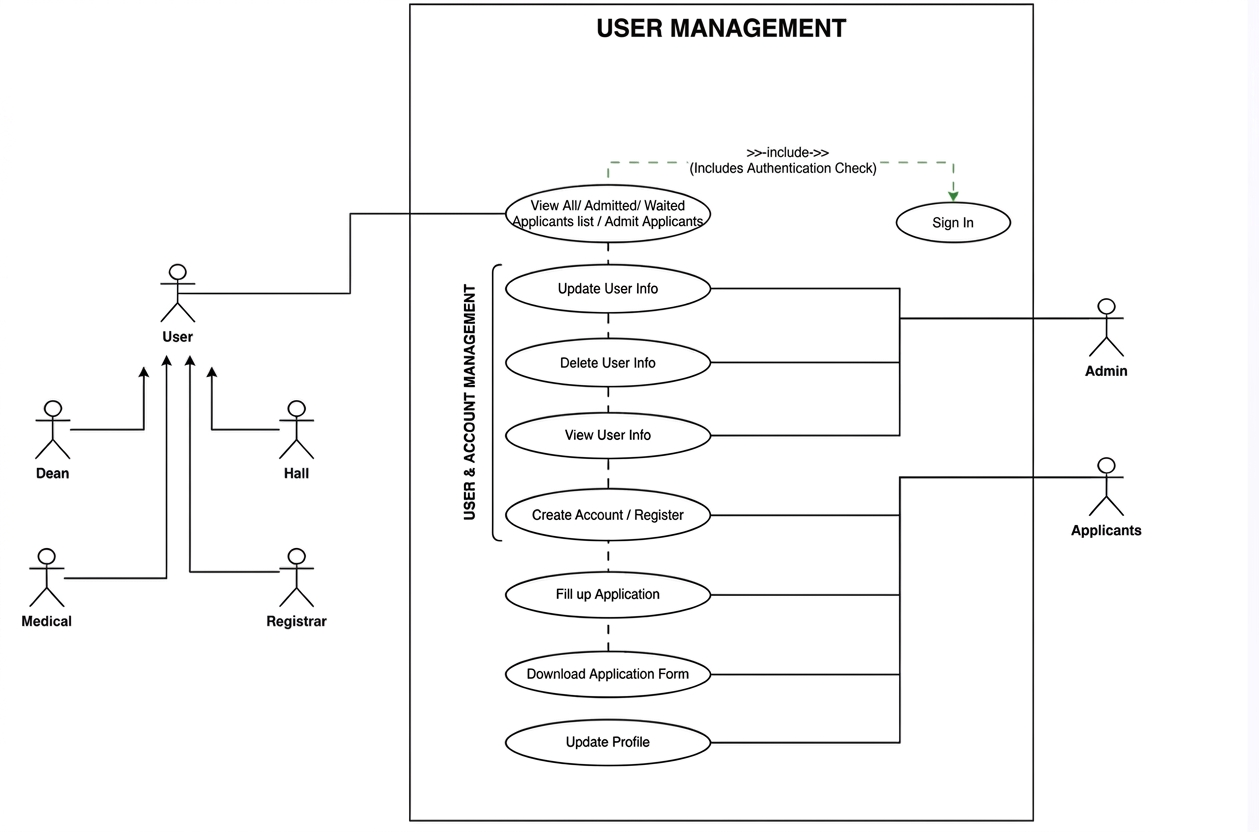
\includegraphics[width=0.85\textwidth]{user.png} 
    \caption{Use Case Diagram of User Management}
    \label{fig:user_management_usecase}
\end{figure}

The User Management use case diagram consists of six primary actors: Admin, Dean Office, Hall Office, Medical Office, Registrar Office, and Applicant. 

\subsubsection{Login Process}

This use case explains how users log into the \textit{Digital Admission Procedure Management for Post-GST Candidates}. It ensures that only authorized users such as staff members and applicants can access the system and its features.

\begin{table}[htbp]
    \centering
    \small
    \renewcommand{\arraystretch}{1.5}
    \caption{Use Case Table: Login Process (UC-1.1)} % ক্যাপশন উপরে আনা হয়েছে
    \label{tab:use_case_login}
    \begin{tabularx}{\textwidth}{|l|X|}
        \hline
        \rowcolor[gray]{0.9} \textbf{Characteristics} & \textbf{Description} \\ \hline
        Use Case ID & UC-1.1 \\ \hline
        Use Case Name & Login Process \\ \hline
        Primary Actors & Admin, Dean Office, Hall Office, Medical Office, Registrar Office, Applicant \\ \hline
        Purpose & To allow users to securely access the system dashboard. \\ \hline
        Precondition & The user must have a valid account with a username or email and password. \\ \hline
        Post-condition & The user is redirected to their respective dashboard based on their role. \\ \hline
        Trigger & The user tries to access a protected page or clicks on the login option. \\ \hline
        Scenario & 
        \begin{enumerate}[nosep, leftmargin=*]
            \item The user opens the login page of the system.
            \item The user enters their username or email along with the password.
            \item The user clicks the Login button.
            \item The system checks the entered information with the PostgreSQL database using Next.js and Prisma.
            \item If the information is correct, a secure session is created.
            \item The user is then allowed to enter the dashboard.
        \end{enumerate} \\ \hline
        Exception & \textbf{Invalid Credentials:} If the entered information is incorrect, the system shows an "Access Denied" message. \\ \hline
        Frequency of Use & Very High (used daily). \\ \hline
    \end{tabularx}
\end{table}
\FloatBarrier
\subsubsection{View Applicant List}

This use case describes the procedure for administrative actors to access and review the records of candidates who have applied for admission.

\begin{table}[htbp]
    \centering
    \caption{Use Case Table: View Applicant List (UC-1.2)}
    \label{tab:view_applicant_list}
    \renewcommand{\arraystretch}{1.5}
    \begin{tabularx}{\textwidth}{|l|X|}
        \hline
        \rowcolor[gray]{0.9} \textbf{Characteristics} & \textbf{Description} \\ \hline
        Use Case ID & UC-1.2 \\ \hline
        Use Case Name & View Applicant List \\ \hline
        Primary Actors & Admin, Dean Office, Hall Office, Medical Office, Registrar Office \\ \hline
        Goal in Context & To filter and view different applicant categories (All, Admitted, or Waiting). \\ \hline
        Precondition & The user must be securely authenticated and signed into the administrative dashboard. \\ \hline
        Triggers & Need to verify candidate status or proceed with departmental clearance. \\ \hline
        Scenario & 
        \begin{enumerate}[nosep, leftmargin=*]
            \item Visit the Dashboard after successful login.
            \item Click on the 'Applicant Management' or 'List' option from the sidebar.
            \item Choose the specific list category (e.g., All Applicants, Admitted List, or Waiting List).
            \item System fetches data from the PostgreSQL database through Prisma and displays the list.
        \end{enumerate} \\ \hline
        Exception & \textbf{Invalid Role:} Access denied if the user lacks sufficient permissions. \\ \hline
        Frequency of Use & High frequency. \\ \hline
    \end{tabularx}
\end{table}
\subsubsection{Update User Information}

This use case describes the administrative process of modifying existing user data within the system. It ensures that the Admin can maintain accurate records for all institutional roles.

\begin{table}[htbp]
    \centering
    \caption{Use Case Table: Update User Information (UC-1.3)}
    \label{tab:update_user_info}
    \renewcommand{\arraystretch}{1.5}
    \begin{tabularx}{\textwidth}{|l|X|}
        \hline
        \rowcolor[gray]{0.9} \textbf{Characteristics} & \textbf{Description} \\ \hline
        Use Case ID & UC-1.3 \\ \hline
        Use Case Name & Update User Information \\ \hline
        Primary Actors & Admin \\ \hline
        Goal in Context & To modify or correct the information of any registered user. \\ \hline
        Precondition & Admin must be securely authenticated and signed into the dashboard. \\ \hline
        Triggers & Requirement to update credentials, roles, or personal details of a user. \\ \hline
        Scenario & 
        \begin{enumerate}[nosep, leftmargin=*]
            \item Visit the Admin dashboard.
            \item Search and select the specific user from the user management list.
            \item Update the necessary information in the provided fields.
            \item Click the \textbf{Update} button.
            \item System performs backend validation and updates the PostgreSQL database via Prisma.
        \end{enumerate} \\ \hline
        Exception & \textbf{Invalid Role:} Attempted access by a non-admin user; \textbf{Validation Error:} Duplicate unique fields. \\ \hline
        Frequency of Use & High frequency. \\ \hline
    \end{tabularx}
\end{table}
\subsubsection{Delete User Information}

This use case describes the administrative process of permanently removing a user's record from the \textit{JUST Undergraduate Final Admission System}. It allows the Admin to maintain system integrity by deleting redundant, unauthorized, or incorrect accounts from the database.

\begin{table}[htbp]
    \centering
    \caption{Use Case Table: Delete User Information (UC-1.4)}
    \label{tab:use_case_delete_user}
    \renewcommand{\arraystretch}{1.5}
    \begin{tabularx}{\textwidth}{|l|X|}
        \hline
        \rowcolor[gray]{0.9} \textbf{Characteristics} & \textbf{Description} \\ \hline
        Use Case ID & UC-1.4 \\ \hline
        Use Case Name & Delete User Information \\ \hline
        Primary Actors & Admin \\ \hline
        Goal in Context & To permanently remove a specific user record from the system database. \\ \hline
        Precondition & The Admin must be signed in and authorized with administrative privileges. \\ \hline
        Post-condition & The user record is successfully removed from the PostgreSQL database via Prisma. \\ \hline
        Triggers & Admin identifies an account that needs to be removed for maintenance or security reasons. \\ \hline
        Scenario & 
        \begin{enumerate}[nosep, leftmargin=*]
            \item The Admin navigates to the \textbf{User Management} section in the dashboard.
            \item The system fetches the list of all registered users.
            \item The Admin identifies and selects the specific user to be deleted.
            \item The Admin clicks the \textbf{Delete} button associated with the user.
            \item A confirmation modal appears to prevent accidental deletion.
            \item Upon confirmation, the backend executes the delete query.
            \item The system updates the UI and displays a success notification.
        \end{enumerate} \\ \hline
        Exception & \textbf{Deletion Failed:} If the user is linked to critical active records, the system prevents deletion and shows a "Constraint Error." \\ \hline
        Frequency of Use & Low to Medium (As needed for system cleanup). \\ \hline
    \end{tabularx}
\end{table}
\subsubsection{View User Information}

This use case allows the Admin to view detailed profiles and access levels of all users (Applicants and Staff) registered within the system.

\begin{table}[htbp]
    \centering
    \caption{Use Case Table: View User Information (UC-1.5)}
    \label{tab:view_user_info}
    \renewcommand{\arraystretch}{1.5}
    \begin{tabularx}{\textwidth}{|l|X|}
        \hline
        \rowcolor[gray]{0.9} \textbf{Characteristics} & \textbf{Description} \\ \hline
        Use Case ID & UC-1.5 \\ \hline
        Use Case Name & View User Information \\ \hline
        Primary Actors & Admin \\ \hline
        Goal in Context & To display the full profile details and role of a specific user. \\ \hline
        Precondition & Admin must be logged into the system with valid credentials. \\ \hline
        Triggers & Need to verify user credentials or check account status. \\ \hline
        Scenario & 
        \begin{enumerate}[nosep, leftmargin=*]
            \item Visit the Admin dashboard.
            \item Navigate to the 'User Management' or 'View Users' section.
            \item Search for a specific user by ID or Email.
            \item Click on the user's profile to see detailed information.
            \item System fetches data from PostgreSQL and displays it on the UI.
        \end{enumerate} \\ \hline
        Exception & \textbf{Invalid Role:} Non-admin users attempting to access this section; Database error. \\ \hline
        Frequency of Use & High frequency. \\ \hline
    \end{tabularx}
\end{table}
\subsubsection{Fill-up Application Form}

This use case outlines the process for a registered applicant to submit their academic and personal details through the \textit{JUST Undergraduate Final Admission System}. It is a multi-step procedure designed to collect necessary documentation and information required for the final admission validation.

\begin{table}[htbp]
    \centering
    \caption{Use Case Table: Fill-up Application Form (UC-1.6)}
    \label{tab:use_case_fillup_form}
    \renewcommand{\arraystretch}{1.5}
    \begin{tabularx}{\textwidth}{|l|X|}
        \hline
        \rowcolor[gray]{0.9} \textbf{Characteristics} & \textbf{Description} \\ \hline
        Use Case ID & UC-1.6 \\ \hline
        Use Case Name & Fill-up Application Form \\ \hline
        Primary Actors & Applicant \\ \hline
        Goal in Context & To successfully submit the complete admission application form. \\ \hline
        Precondition & The applicant must be signed in and should not have a previously submitted pending application. \\ \hline
        Post-condition & The application data is stored in the database, and the status is set to "Pending" for office review. \\ \hline
        Triggers & Applicant clicks on the "Apply Now" or "Fill-up Form" button on their dashboard. \\ \hline
        Scenario & 
        \begin{enumerate}[nosep, leftmargin=*]
            \item The applicant navigates to the application form section.
            \item The system presents a multi-step form (Personal Info, Academic History, Document Upload).
            \item The applicant enters all required information and uploads necessary files (Photo, Signature, etc.).
            \item The applicant reviews the information for any errors.
            \item The applicant clicks the \textbf{Submit} button.
            \item The Next.js frontend sends the data to the API, which persists it in PostgreSQL via Prisma.
            \item A success confirmation message is displayed to the applicant.
        \end{enumerate} \\ \hline
        Exception & \textbf{Validation Error:} If required fields are empty or files are in an unsupported format, the system prompts the user to correct the errors. \\ \hline
        Frequency of Use & Once per applicant (High volume during admission periods). \\ \hline
    \end{tabularx}
\end{table}
\subsubsection{Download Application Form}

This use case provides the applicant with the ability to generate and download a formal PDF version of their submitted application. It serves as an official record for the applicant, which is essential for the physical verification process at \textit{Jashore University of Science and Technology (JUST)}.

\begin{table}[!htbp]
    \centering
    \small
    \renewcommand{\arraystretch}{1.4}
    \begin{tabularx}{\textwidth}{|l|X|}
        \hline
        \rowcolor[gray]{0.9} \textbf{Characteristics} & \textbf{Description} \\ \hline
        Use Case ID & UC-1.7 \\ \hline
        Use Case Name & Download Application Form \\ \hline
        Primary Actors & Applicant \\ \hline
        Goal in Context & To obtain a digital or physical copy of the completed admission form for official documentation. \\ \hline
        Precondition & The applicant must be securely signed in and must have successfully submitted their admission application. \\ \hline
        Post-condition & A PDF document is dynamically generated and successfully downloaded to the applicant's local device. \\ \hline
        Triggers & The applicant clicks the \textbf{Download PDF} or \textbf{Print Application} button on their personal dashboard. \\ \hline
        Scenario & 
        \begin{enumerate}[nosep, leftmargin=*]
            \item The applicant navigates to their personal dashboard.
            \item The system verifies the application status from the PostgreSQL database.
            \item The applicant clicks the \textbf{Download PDF} button.
            \item The Next.js server-side logic triggers the PDF generation engine using the applicant's stored data.
            \item The system initiates the file download stream in the user's browser.
            \item The applicant saves the generated PDF file for future reference and physical submission.
        \end{enumerate} \\ \hline
        Exception & \textbf{Generation Error:} If there is a server-side failure or the database is unreachable, a "PDF Generation Failed" error is displayed. \\ \hline
        Frequency of Use & High (Once per applicant after the successful submission of the form). \\ \hline
    \end{tabularx}
    
    \caption{Use Case Table: Download Application Form (UC-1.7)}
    \label{tab:use_case_download_form}
\end{table}
\FloatBarrier

% --- DEAN OFFICE MANAGEMENT ---
\subsection{Dean Office Management}

\begin{figure}[htbp]
    \centering
    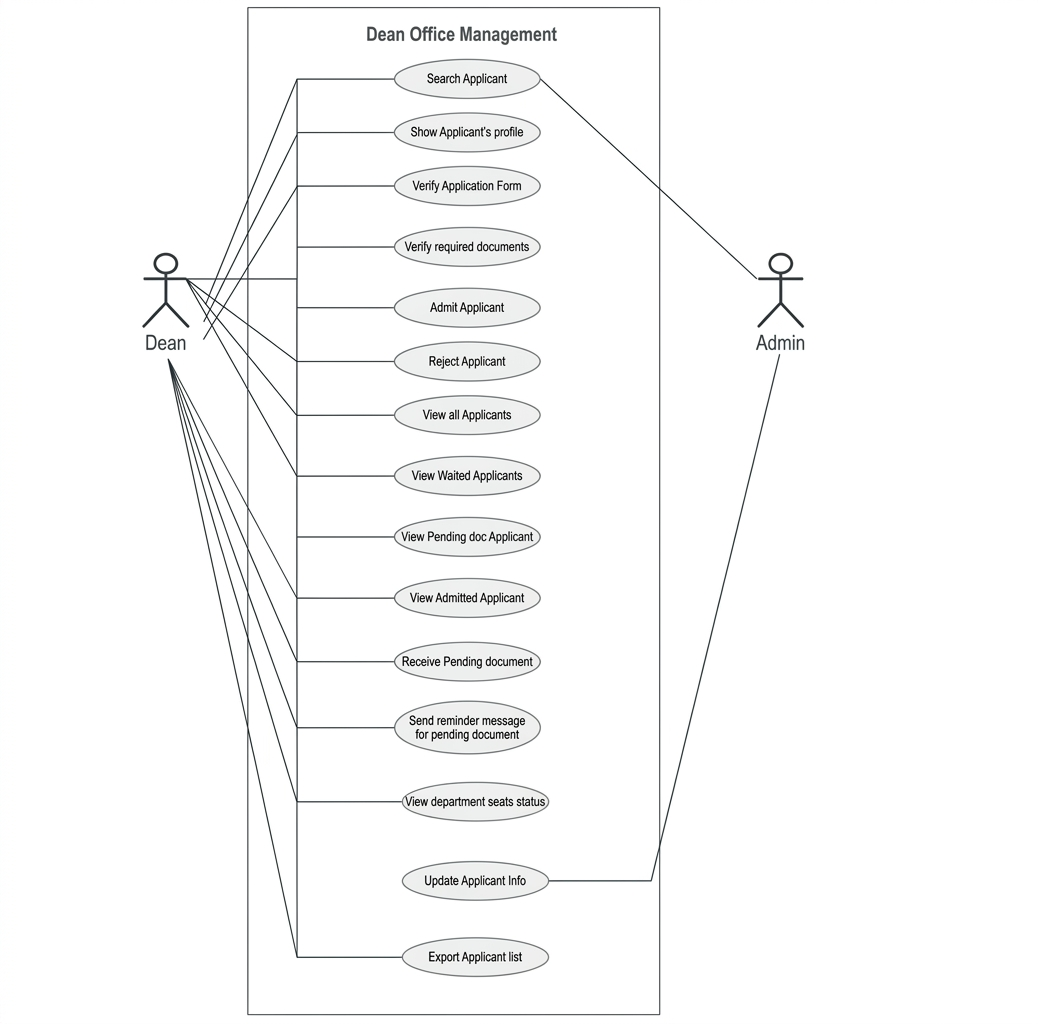
\includegraphics[width=0.85\textwidth]{dean.png}
    \caption{Use Case Diagram of Dean Office Management}
    \label{fig:dean_usecase}
\end{figure}

The Dean Office Management use case diagram consists of two primary actors: Admin and Dean Office. 
This module controls various types of use cases including searching applicants, viewing applicant profiles, verifying application forms, verifying required documents, admitting applicants, rejecting applicants, and managing applicant lists. It also provides functionalities to view all applicants, waited applicants, and admitted applicants with or without pending documents. 

\subsubsection{Applicant Search}


In this use case, you will learn about how the Dean Office uses the system to find a particular applicant. This makes it possible for those authorized to find applicant records through the search parameter like application number, name, or registration number. This feature ensures that there is a reduced workload on the side of the Dean Office whenever it involves searching for numerous admission records. By applying this functionality, the Dean Office can view all academic and personal details entered during the application process. It should be noted that there is a provision for sorting and filtering results from the search. This makes it possible to view accurate results.

\begin{table}[!htbp]
    \centering
    \small
    \renewcommand{\arraystretch}{1.5}
    % ক্যাপশন এবং লেবেল উপরে সেট করা হয়েছে
    \caption{Use Case Table: Applicant Search (UC-2.1)}
    \label{tab:dean_search}
    
    \begin{tabularx}{\textwidth}{|l|X|}
        \hline
        \rowcolor[gray]{0.9} {Characteristics} & {Description} \\ \hline
        Use Case ID & UC-2.1 \\ \hline
        Use Case Name & Applicant Search \\ \hline
        Actors & Dean Office \\ \hline
        Goal Statement & To conduct a search for a specific applicant using Applicant ID or Roll. \\ \hline
        Preconditions & The user must be logged in and have the Applicant ID or Roll. \\ \hline
        Trigger & The need to find information about a particular applicant. \\ \hline
        Steps &
        \begin{enumerate}[nosep, leftmargin=*]
        \item Navigate to the Dean Office dashboard.
        \item Enter the Applicant ID or Roll in the search field.
        \item Press Enter to perform the search.
        \end{enumerate} \\ \hline
        Exceptions & Invalid role. \\ \hline
        Occurrence & Very frequent \\ \hline
    \end{tabularx}
\end{table}
\FloatBarrier
\subsubsection{Display Applicant Profile}

This use case describes how the Dean Office views the profile of an applicant. 
It provides a complete view of the applicant’s personal and academic information, 
which helps in the admission process.

\begin{table}[!htbp]
    \centering
    \small
    \renewcommand{\arraystretch}{1.4}
    % ক্যাপশন এবং লেবেল উপরে সেট করা হয়েছে
    \caption{Use Case Table: Display Applicant Profile (UC-2.2)}
    \label{tab:dean_profile}
    
    \begin{tabularx}{\textwidth}{|l|X|}
        \hline
        \rowcolor[gray]{0.9} \textbf{Features} & \textbf{Description} \\ \hline
        Use Case ID & UC-2.2 \\ \hline
        Use Case Name & Display Applicant Profile \\ \hline
        Actors & Dean Office \\ \hline
        Goal Statement & To display the detailed profile of the selected applicant for assessment purposes. \\ \hline
        Precondition & The user should be logged in and must have searched for the applicant. \\ \hline
        Postcondition & The applicant data will be shown on the screen from the PostgreSQL database using Prisma ORM. \\ \hline
        Trigger & When there is a need to view personal or academic information of an applicant during the admission process. \\ \hline
        Steps & 
        \begin{enumerate}[nosep, leftmargin=*]
            \item Search for a particular applicant from the applicant list.
            \item Click on the \textbf{Profile} or \textbf{Details} button.
            \item The system retrieves the applicant’s data.
            \item The system displays the applicant information on the screen.
        \end{enumerate} \\ \hline
        Exception & Data not available: An error message will be shown. Access forbidden: The user cannot view the data. \\ \hline
        Frequency & High (When the admission process is underway) \\ \hline
    \end{tabularx}
\end{table}
\FloatBarrier
\subsubsection{Verify Application Form}

This use case describes the procedure for the Dean Office to verify the submitted application form. It ensures that the applicant's data and uploaded documents are consistent with the university's requirements before granting final approval.

\begin{table}[!htbp]
    \centering
    \small
    \renewcommand{\arraystretch}{1.4}
    \begin{tabularx}{\textwidth}{|l|X|}
        \hline
        \rowcolor[gray]{0.9} \textbf{Characteristics} & \textbf{Description} \\ \hline
        Use Case ID & UC-2.3 \\ \hline
        Use Case Name & Verify Application Form \\ \hline
        Primary Actors & Dean Office \\ \hline
        Goal in Context & To successfully validate and approve the applicant's submitted application form. \\ \hline
        Precondition & The user must be signed in with Dean Office privileges and an application must be pending review. \\ \hline
        Post-condition & The application status is updated to 'Verified' in the PostgreSQL database and reflected on the system. \\ \hline
        Triggers & Requirement to process and authorize candidate applications for the final admission list. \\ \hline
        Scenario & 
        \begin{enumerate}[nosep, leftmargin=*]
            \item The user searches for a specific applicant record from the pending list.
            \item The user navigates to the \textbf{Verification} or \textbf{Review} section.
            \item The system displays the submitted data and documents via the interface.
            \item The user reviews the information and clicks the \textbf{Approve} or \textbf{Verify} button.
            \item The system updates the status using Prisma ORM.
        \end{enumerate} \\ \hline
        Exception & \textbf{Data Mismatch:} If the information is incorrect, the user may reject the form or request a correction from the applicant. \\ \hline
        Frequency of Use & High (During peak admission cycles). \\ \hline
    \end{tabularx}
    \caption{Use Case Table: Verify Application Form (UC-2.3)}
    \label{tab:dean_verify_form}
\end{table}
\FloatBarrier
\subsubsection{Verify Required Documents}

In this use case, the Dean Office verifies the uploaded physical documents of an applicant, ensuring that all the academic certificates and other necessary papers are genuine and satisfy the university requirements.

\begin{table}[!htbp]
    \centering
    \small
    \renewcommand{\arraystretch}{1.4}
    \begin{tabularx}{\textwidth}{|l|X|}
        \hline
        \rowcolor[gray]{0.9} \textbf{Characteristics} & \textbf{Description} \\ \hline
        Use Case ID & UC-2.4 \\ \hline
        Use Case Name & Verify Required Documents \\ \hline
        Primary Actor & Dean Office \\ \hline
        Purpose of Use Case & To ensure the successful verification and confirmation of the applicant’s documents. \\ \hline
        Precondition & User must be logged in, and the applicant’s records must be accessed. \\ \hline
        Post-Condition & Document status changes to “Verified” in the PostgreSQL database. \\ \hline
        Trigger & Initiation of the process of verifying documents during the admission process. \\ \hline
        Scenario Steps & 
        \begin{enumerate}[nosep, leftmargin=*]
            \item Step 1: Search for a particular applicant from the dashboard.
            \item Step 2: Go to the Verify Required Documents tab.
            \item Step 3: Choose specific documents submitted by the candidate.
            \item Step 4: Click Verify to confirm using Prisma ORM.
        \end{enumerate} \\ \hline
        Exceptions & Invalid Role: Unapproved personnel tries to perform verification. Missing Docs: System raises an alert due to missing documents. \\ \hline
        Frequency of Use & Very high \\ \hline
    \end{tabularx}
    \caption{Table of Use Case: Verify Required Documents (UC-2.4)}
    \label{tab:dean_verify_docs}
\end{table}
\FloatBarrier
\subsubsection{Admit Applicant (Dean Clearance)}

The use case gives the Dean Office the ability to provide final clearance for admission after successful verification of all records.Furthermore, the system ensures that the final clearance is only provided if allnecessary verification steps have been completed successfully. This allows the Dean Office to see a comprehensive report on the applicant’s academic, medical, and administrative records, before issuing its final approval. It also includes an interface which helps in either accepting or rejecting the decision along with proper justification. As soon as the clearance is provided, the system makes automatic changes to the status of the applicant in all the modules. This means that the applicant will not be able to make any further changes to the approved application without valid permission from relevant authorities. In addition, it creates an entry for final approval so as to keep record for future references. It also sends notification to the applicant, once the final decision is made. The proposed work flow prevents applicants from skipping any step during their verification process. Also, there is no need for manual verification as the system automatically makes changes in other modules.
\begin{table}[H]
    \centering
    \small
    \renewcommand{\arraystretch}{1.4}
    % ক্যাপশন এবং লেবেল উপরে সেট করা হয়েছে
    \caption{Use Case Table 2.12: UC-2.5}
    \label{tab:dean_admit}
    
    \begin{tabularx}{\textwidth}{|l|X|}
        \hline
        \rowcolor[gray]{0.9} {Characteristics} & {Description} \\ \hline
        Use Case ID & UC-2.5 \\ \hline
        Name of Use Case & Admit Applicant \\ \hline
        Main Actors & Dean Office \\ \hline
        Goal & The goal of the use case is to allow admission clearance of the applicant. \\ \hline
        Precondition & Documents should be verified, and the applicant should be eligible. \\ \hline
        Post Condition & The applicant is set as “Admitted,” while the seats in the department are increased. \\ \hline
        Steps & 
        \begin{enumerate}[nosep, leftmargin=*]
            \item Find the eligible record of the applicant.
            \item Read the final summary of the candidate.
            \item Press the Admit button.
            \item Record is saved in PostgreSQL database.
        \end{enumerate} \\ \hline
        Exceptions & Full seat or unauthorized role. \\ \hline
        Usage Frequency & Very Frequent \\ \hline
    \end{tabularx}
\end{table}
\FloatBarrier
\subsubsection{Decline Applicant}

This use case outlines how to decline an applicant in case discrepancies exist in their documentation or eligibility.

\begin{table}[!htbp]
    \centering
    \small
    \renewcommand{\arraystretch}{1.4}
    % ক্যাপশন এবং লেবেল উপরে সেট করা হয়েছে
    \caption{Use Case Table: Decline Applicant (UC-6.2)}
    \label{tab:dean_decline}
    
    \begin{tabularx}{\textwidth}{|l|X|}
        \hline
        \rowcolor[gray]{0.9} \textbf{Characteristic} & \textbf{Description} \\ \hline
        Use Case ID & UC-2.6 \\ \hline
        Use Case Name & Decline Applicant \\ \hline
        Primary Actors & Dean’s Office \\ \hline
        Goal in Context & The goal is to exclude an applicant due to mistakes or violations. \\ \hline
        Steps & 
        \begin{enumerate}[nosep, leftmargin=*]
            \item Locate the relevant applicant.
            \item Click on the Decline button.
            \item Give a reason for declining the application (optional/mandatory).
            \item The system marks the application as “Declined.”
        \end{enumerate} \\ \hline
        Exception & Occurs when unauthorized users decline valid applicants or reject applicants incorrectly. \\ \hline
        Usage Frequency & High \\ \hline
    \end{tabularx}
\end{table}
\FloatBarrier
\subsubsection{Application List Views (All, Waiting, Admittees)}

This use case describes the procedure for how the Dean's office is able to monitor different kinds of applicants using the sidebar menu in the dashboard.The system offers navigation categories that can be used to screen applicants depending on their academic standing and documents submitted.The Dean's office members can conveniently switch between different applicants for the sake of efficiency.Each category shows all the necessary information about the respective applicants in an orderly manner.The dashboard guarantees instant update of the system such that changes in the application standing will always be seen by the Dean's office.It also makes it easier for the Dean's office to track pending, accepted, and denied applications independently.In this way, the verification process becomes more effective.Moreover, the sidebar navigation in the system is created in a way that allows users to switch to various sections effortlessly. The system sorts applicants according to several parameters, including verification status, completeness of submitted documents, and whether there are requirements to fulfill for particular applicants. It will assist in minimizing confusion while working with numerous applications. There are options for fast search and filtration of applicants in each section. Visual markers such as statuses and color codes can be used to indicate the current status of each application, which will make it easier for the Dean's office to see applications that need more attention.The system includes the real-time synchronization function so that changes made in applications by other offices are immediately visible from the dashboard. It helps avoid misunderstandings and miscommunications between offices as well as inconsistency. In addition, the sidebar navigation makes it possible to easily switch between various workflow stages to increase overall productivity. User activity can be recorded in the system so that it can be used to track the decision-making process later on.

\begin{table}[H]
    \centering
    \small
    \renewcommand{\arraystretch}{1.4}
    % ক্যাপশন উপরে সেট করা হয়েছে
    \caption{Use Case Table: Application List Management (UC-2.7 - 2.9)}
    \label{tab:app_list_management}
    
    \begin{tabularx}{\textwidth}{|l|X|}
        \hline
        \rowcolor[gray]{0.9} {Characteristic} & {Explanation} \\ \hline
        Use Case Number & UC-2.7, 2.8, 2.9 \\ \hline
        Name of Use Case & View All, Waiting \& Admitted Applicants \\ \hline
        Actors & Dean’s Office \\ \hline
        Steps & 
        \begin{enumerate}[nosep, leftmargin=*]
            \item Login to the Dean’s Dashboard.
            \item Select the specific type (All / Waiting / Admitted).
            \item The system will then search for relevant information in the PostgreSQL database through Prisma.
        \end{enumerate} \\ \hline
        Frequency of Use & High \\ \hline
    \end{tabularx}
\end{table}
\FloatBarrier
\subsubsection{Pending Documents and Reminders}

This use case involves collecting pending documents and issuing reminders to those applicants who have yet to provide complete documents.
The application will identify those applicants that are lacking or having incomplete documentation in the process of verification. 
An automatic list of applicants with incomplete documentation will be created by the system.
The reminders could be issued to the concerned applicants using the system’s interface by authorized personnel. 
Through reminders, the applicant will come to know which documents he/she needs to supply in order to complete his/her application. 
The reminders could also keep a record as to whether the applicants responded to the reminders or not.

\begin{table}[H]
    \centering
    \small
    \renewcommand{\arraystretch}{1.4}
    % ক্যাপশন উপরে সেট করা হয়েছে
    \caption{Use Case Table: Pending Documents Management (UC-2.11 - 2.13)}
    \label{tab:pending_docs_mgmt}
    
    \begin{tabularx}{\textwidth}{|l|X|}
        \hline
        \rowcolor[gray]{0.9} {Characteristic} & {Description} \\ \hline
        Use Case ID & UC-2.11, 2.12, 2.13 \\ \hline
        Use Case Name & Manage Pending Documents \& Send Reminders \\ \hline
        Primary Actor & Dean Office \\ \hline
       Reminders Reminder Scenario: &
\begin{enumerate}[nosep, leftmargin=*]
	\item Locate the applicants whose documents are incomplete.
	\item Identify the particular incomplete documents for each applicant.
	\item Pick the necessary documents and click on Send Message.
	\item A notification alert will be sent by the system to the applicant.
	\item Reminder status will be updated once notification alert is sent.
	\item The system will save the reminder history for any future use.
	\item The dean office can re-notify the applicant if the application does not respond to the notification.
\end{enumerate} \\ \hline 

Receive Documents: & 
\begin{enumerate}[nosep, leftmargin=*]
	\item Open the Action Pending Documents on the side bar menu.
	\item Crosscheck the submitted physical documents.
	\item Update the status of the documents that were successfully checked.
	\item Register the receipt of the missing documents.
	\item Update the verification status of the applicant automatically.
	\item Save the updated information for auditing purposes.
\end{enumerate} \\ \hline
    \end{tabularx}
\end{table}
\FloatBarrier
\subsubsection{Seats Status and Data Export}

\begin{table}[!htbp]
    \centering
    \small
    \renewcommand{\arraystretch}{1.4}
    \begin{tabularx}{\textwidth}{|l|X|}
        \hline
        \rowcolor[gray]{0.9} \textbf{Characteristics} & \textbf{Description} \\ \hline
        Use Case ID & UC-2.14, 2.15 \\ \hline
        Use Case Name & View Seats Status \& Export Lists \\ \hline
        Primary Actors & Dean \\ \hline
        Goal in Context & To monitor enrollment capacity and generate reports in CSV/Excel format. \\ \hline
        Scenario (Export) & 
        \begin{enumerate}[nosep, leftmargin=*]
            \item Navigate to the desired applicant list.
            \item Click the \textbf{Export} button.
            \item The system generates and downloads the file.
        \end{enumerate} \\ \hline
    \end{tabularx}
    \caption{Use Case Table: Monitoring and Export (UC-2.14 - 2.15)}
\end{table}
\FloatBarrier

% --- HALL OFFICE MANAGEMENT ---
\subsection{Hall Office Management}

\begin{figure}[htbp]
    \centering
    \begin{tikzpicture}[
    node distance = 1cm and 2cm,
    actor/.style={scale=0.5},
    usecase/.style={ellipse, draw, minimum width=4cm, minimum height=0.7cm, align=center, font=\small},
    link/.style={draw, thick}
]
% System Boundary
\draw[thick] (0, 0) rectangle (9, -12);
\node at (4.5, -0.5) {{Hall Office Management}};

% Actors
\node (hallAuth) at (-2, -5.5) {
    \begin{tikzpicture}[scale=0.5]
        \draw[thick] (0,1.2) circle (0.4cm); \draw[thick] (0,0.8) -- (0,-0.8);
        \draw[thick] (-0.8,0.4) -- (0.8,0.4); \draw[thick] (0,-0.8) -- (-0.5,-1.8); \draw[thick] (0,-0.8) -- (0.5,-1.8);
        \node at (0,-2.5) {\small Hall Authority};
    \end{tikzpicture}
};

\node (admin) at (11, -5.5) {
    
\begin{tikzpicture}[scale=0.5]
        \draw[thick] (0,1.2) circle (0.4cm); \draw[thick] (0,0.8) -- (0,-0.8);
        \draw[thick] (-0.8,0.4) -- (0.8,0.4); \draw[thick] (0,-0.8) -- (-0.5,-1.8); \draw[thick] (0,-0.8) -- (0.5,-1.8);
        \node at (0,-2.5) {\small Admin};
    \end{tikzpicture}
};

% Use Cases
\node[usecase] (uc1) at (4.5, -1.5) {Search Applicant};
\node[usecase] (uc2) at (4.5, -2.5) {Show Applicant Profile};
\node[usecase] (uc3) at (4.5, -3.5) {Receive Bank Receipt};
\node[usecase] (uc4) at (4.5, -4.5) {Admit Applicant};
\node[usecase] (uc5) at (4.5, -5.5) {View Waited Applicants};
\node[usecase] (uc6) at (4.5, -6.5) {View Admitted Applicants};
\node[usecase] (uc7) at (4.5, -7.5) {Update Applicant Info};
\node[usecase] (uc8) at (4.5, -8.5) {Download Official Record};
\node[usecase] (uc9) at (4.5, -9.5) {Export Admitted List};

% Connections
\foreach \i in {uc1,uc2,uc3,uc4,uc5,uc6,uc8,uc9} \draw[link] (hallAuth) -- (\i.west);
\draw[link] (admin) -- (uc7.east);
\draw[link] (admin) -- (uc4.east);
\end{tikzpicture}
    \caption{Use Case Diagram of Hall Office Management}
    \label{fig:hall_usecase}
\end{figure}

The Hall Office Management use case diagram consists of two primary actors: Admin and Hall Authority. This module handles various operations including searching applicants, admitting them after bank receipt verification, managing lists, and updating information.

\subsubsection{Search for Applicant}

In this use case, the Hall Office will be able to conduct searches for applicant data using either the GST ID or the roll number of the applicant. This feature makes it easy for one to be able to get the applicant's data within a short time.Moreover, the system helps display the results in a systematic way, which allows the Hall Office to easily find the right candidate from amongst all those who have applied. The system makes the process of data search much easier and faster for the Hall Office. The search feature also helps minimize any risk of errors as the records can be easily identified using GST ID or roll numbers. Another advantage of the search functionality of the system is that it gives the Hall Office immediate access to all the information about each and every applicant.

\begin{table}[H]
    \centering
    \small
    \renewcommand{\arraystretch}{1.4} 
    \caption{Use Case Table: Search Applicant (UC-3.1)} % ক্যাপশন উপরে আনা হয়েছে
    \label{tab:search-applicant}
    \begin{tabularx}{\textwidth}{|l|X|}
        \hline
        \rowcolor[gray]{0.9} {Description of Characteristics} & {Details} \\ \hline
        Use Case ID & UC-3.1 \\ \hline
        Use Case Name & Search Applicant \\ \hline
        Actors & Hall Office \\ \hline
        Purpose & To locate an applicant’s details in the system. \\ \hline
        Pre-condition & The user must be logged into the system and have the GST Applicant ID or Roll. \\ \hline
        Scenarios & 
        \begin{enumerate}[nosep, leftmargin=*, after=\vspace{-\baselineskip}, before=\vspace{-0.5\baselineskip}]
            \item User navigates to the Hall Office dashboard.
            \item User enters the GST ID or Roll Number.
            \item System fetches and displays the applicant details.
        \end{enumerate} \\ \hline
        Occurrence & Often \\ \hline
    \end{tabularx}
\end{table}
\FloatBarrier
\subsubsection{Show Applicant Profile}
\begin{table}[!htbp]
    \centering\small\renewcommand{\arraystretch}{1.4}
    \begin{tabularx}{\textwidth}{|l|X|}
        \hline \rowcolor[gray]{0.9} \textbf{Characteristics} & \textbf{Description} \\ \hline
        Use Case ID & UC-3.2 \\ \hline
        Use Case Name & Show Applicant Profile \\ \hline
        Primary Actors & Hall Office \\ \hline
        Goal & Display detailed academic and personal information. \\ \hline
        Scenario & 1. Search applicant. 2. Click 'Profile' button. \\ \hline
    \end{tabularx}
    \caption{Use Case: Show Applicant Profile (UC-3.2)}
\end{table}
\FloatBarrier
\subsubsection{Receive Bank Receipt}
This use case enables the Hall Office to collect and validate the applicant's bank receipt for their hall fees. The purpose is to ensure that the payment has been made either manually or digitally. Once the receipt is validated, the applicant's payment status will be updated in the system.
\begin{table}[H]
    \centering
    \small
    \renewcommand{\arraystretch}{1.4}
    \caption{Use Case: Receive Bank Receipt (UC-3.3)} % ক্যাপশন এখন উপরে
    \label{tab:receive-bank-receipt}
    \begin{tabular}{|l|p{10cm}|} 
        \hline
        \rowcolor[gray]{0.9} {Characteristics} & {Description} \\ \hline
        Use Case ID & UC-3.3 \\ \hline
        Use Case Name & Receive Bank Receipt \\ \hline
        Primary Actors & Hall Office \\ \hline
        Goal & To confirm the physical or electronic copy of hall fees. \\ \hline
        Scenario & 1. Find the applicant. 2. Click 'Receive Receipt' button. 3. The system will update PostgreSQL database using Prisma. \\ \hline
    \end{tabular}
\end{table}
\FloatBarrier
\subsubsection{Admit Applicant (Hall Clearance)}
\begin{table}[!htbp]
    \centering\small\renewcommand{\arraystretch}{1.4}
    \begin{tabularx}{\textwidth}{|l|X|}
        \hline \rowcolor[gray]{0.9} \textbf{Characteristics} & \textbf{Description} \\ \hline
        Use Case ID & UC-3.4 \\ \hline
        Use Case Name & Admit Applicant (Hall Clearance) \\ \hline
        Primary Actors & Hall Office \\ \hline
        Goal & Grant clearance for final admission. \\ \hline
        Scenario & 1. Verify receipt. 2. Click 'Admit' button. \\ \hline
    \end{tabularx}
    \caption{Use Case: Admit Applicant (UC-3.4)}
\end{table}
\FloatBarrier
\subsubsection{Viewing Lists of Candidates}

This use case is useful for the Hall Administration because it enables the administrators to see lists of candidates who have waited and been admitted. The use case helps in keeping tabs on the status of the applicants at various stages of the admission process. The user is able to access the lists via the sidebar menu.

\begin{table}[H]
    \centering
    \small
    \renewcommand{\arraystretch}{1.4}
    % ক্যাপশন উপরে সেট করা হয়েছে
    \caption{Use Case: Candidate Lists (UC-3.5 – 3.6)}
    \label{tab:candidate_lists_hall}
    
    \begin{tabularx}{\textwidth}{|l|X|}
        \hline
        \rowcolor[gray]{0.9} {Attributes} & {Description} \\ \hline
        Use Case ID & UC-3.5, 3.6 \\ \hline
        Use Case Title & View Waited / Admitted Candidates \\ \hline
        Primary Actor & Hall Administration \\ \hline
        Objective & Track the status of candidates in various stages. \\ \hline
        Scenarios & 1. Move to the sidebar menu. 2. Select the relevant list (Waited/Admitted). \\ \hline
    \end{tabularx}
\end{table}
\FloatBarrier
\subsubsection{Updating Information of Candidates}

\begin{table}[!htbp]
    \centering
    \small
    \renewcommand{\arraystretch}{1.4} % আপনার চাহিদা অনুযায়ী এটি ১.৪ রাখা হয়েছে
    \begin{tabularx}{\textwidth}{|l|X|}
        \hline
        \rowcolor[gray]{0.9} \textbf{Attributes} & \textbf{Description} \\ \hline
        Use Case ID & UC-3.7 \\ \hline
        Use Case Title & Update Candidate Information \\ \hline
        Primary Actor & Administration \\ \hline
        Objective & Modify or correct information for a candidate. \\ \hline
        Scenarios & 1. Click Candidate Table. 2. Change Values. 3. Click Update. \\ \hline
    \end{tabularx}
    \caption{Use Case: Candidate Information (UC-3.7)}
    \label{tab:update-candidate-info}
\end{table}
\FloatBarrier
\subsubsection{Export and Download Records}
\begin{table}[!htbp]
    \centering\small\renewcommand{\arraystretch}{1.4}
    \begin{tabularx}{\textwidth}{|l|X|}
        \hline \rowcolor[gray]{0.9} \textbf{Characteristics} & \textbf{Description} \\ \hline
        Use Case ID & UC-3.8, 3.9 \\ \hline
        Use Case Name & Export List / Download Official Record \\ \hline
        Primary Actors & Hall Office \\ \hline
        Goal & Generate PDF or CSV reports for office records. \\ \hline
        Scenario & 1. Go to list. 2. Click Export/PDF button. \\ \hline
    \end{tabularx}
    \caption{Use Case: Reporting (UC-3.8 - 3.9)}
\end{table}
\FloatBarrier

% --- MEDICAL OFFICE MANAGEMENT ---
\subsection{Medical Office Management}

\begin{figure}[htbp]
    \centering
    \begin{tikzpicture}[
    node distance = 1cm and 2cm,
    usecase/.style={ellipse, draw, minimum width=4.5cm, minimum height=0.7cm, align=center, font=\small},
    link/.style={draw, thick}
]
% Boundary
\draw[thick] (0, 0) rectangle (9, -13.5);
\node at (4.5, -0.6) {\textbf{Medical Office Management}};

% Medical Officer Actor
\node (medOfficer) at (-2, -5.5) {
    \begin{tikzpicture}[scale=0.5]
        \draw[thick] (0,1.2) circle (0.4cm); \draw[thick] (0,0.8) -- (0,-0.8);
        \draw[thick] (-0.8,0.4) -- (0.8,0.4); \draw[thick] (0,-0.8) -- (-0.5,-1.8); \draw[thick] (0,-0.8) -- (0.5,-1.8);
        \node at (0,-2.5) {\small Medical Officer};
    \end{tikzpicture}
};

% Admin Actor
\node (admin) at (11, -5.5) {
    
\begin{tikzpicture}[scale=0.5]
        \draw[thick] (0,1.2) circle (0.4cm); \draw[thick] (0,0.8) -- (0,-0.8);
        \draw[thick] (-0.8,0.4) -- (0.8,0.4); \draw[thick] (0,-0.8) -- (-0.5,-1.8); \draw[thick] (0,-0.8) -- (0.5,-1.8);
        \node at (0,-2.5) {\small Admin};
    \end{tikzpicture}
};

% Use Cases
\node[usecase] (uc1) at (4.5, -1.5) {Search Applicant};
\node[usecase] (uc2) at (4.5, -2.6) {Show Applicant's profile};
\node[usecase] (uc3) at (4.5, -3.7) {Admit Applicant};
\node[usecase] (uc4) at (4.5, -4.8) {View Waited Applicants};
\node[usecase] (uc5) at (4.5, -5.9) {View Admitted Applicant};
\node[usecase] (uc6) at (4.5, -7.0) {Update Applicant Info};
\node[usecase] (uc7) at (4.5, -8.1) {Export Applicant list};
\node[usecase] (uc8) at (4.5, -9.2) {Download Official Record};
\node[usecase] (uc9) at (4.5, -10.3) {Insert/ Update Medical Info};
\node[usecase] (uc10) at (4.5, -11.4) {Generate and print Medical \\ report};

% Left Connections
\foreach \i in {uc1,uc2,uc3,uc4,uc5,uc7,uc8,uc9,uc10} \draw[link] (medOfficer.east) -- (\i.west);

% Right Connections
\draw[link] (admin.west) -- (uc6.east);
\draw[link] (admin.west) -- (uc3.east);
\end{tikzpicture}
    \caption{Use Case Diagram of Medical Office Management}
    \label{fig:medical_usecase}
\end{figure}

The Medical Office Management module handles the physical examination and medical clearance of applicants. This use case diagram involves two primary actors: Medical Officer and Admin. The system allows managing medical records, generating reports, and granting final medical clearance.

\subsubsection{Search Applicant}

\begin{table}[!htbp]
    \centering
    \small
    \renewcommand{\arraystretch}{1.4}
    \caption{Use Case Table: Search Applicant (UC-4.1)} % ক্যাপশন উপরে আনা হয়েছে
    \label{tab:search-applicant-medical}
    \begin{tabularx}{\textwidth}{|l|X|}
        \hline
        \rowcolor[gray]{0.9} \textbf{Characteristics} & \textbf{Description} \\ \hline
        Use Case ID & UC-4.1 \\ \hline
        Use Case Name & Search Applicant \\ \hline
        Primary Actors & Medical Office \\ \hline
        Scenario & 1. Log-in Dashboard. 2. Enter Search Box. 3. Hit Enter. \\ \hline
    \end{tabularx}
\end{table}
\FloatBarrier
\subsubsection{Show Applicant Profile}

\begin{table}[!htbp]
    \centering
    \small
    \renewcommand{\arraystretch}{1.4}
    \begin{tabularx}{\textwidth}{|l|X|}
        \hline
        \rowcolor[gray]{0.9} \textbf{Characteristics} & \textbf{Description} \\ \hline
        Use Case ID & UC-4.2 \\ \hline
        Use Case Name & Show Applicant Profile \\ \hline
        Primary Actors & Medical Office \\ \hline
        Scenario & 1. Search Applicant. 2. Click Profile Button. \\ \hline
    \end{tabularx}
    \caption{Use Case Table: Show Applicant Profile (UC-4.2)}
\end{table}
\FloatBarrier
\subsubsection{Insert/Update Medical Information}
This particular case enables the Medical Office to input or modify the details related to the medical history of an applicant into the system. It will help in assessing the physical fitness of the applicant by making entries in the correct manner. In order to do this, the concerned medical office can complete the necessary form after finding the particular applicant.
\begin{table}[H]
    \centering
    \small
    \renewcommand{\arraystretch}{1.4}
    \caption{Use Case Table: Insert/Update Medical Information (UC-4.3)} % ক্যাপশন উপরে আনা হয়েছে
    \label{tab:medical-info-update}
    \begin{tabularx}{\textwidth}{|l|X|}
        \hline
        \rowcolor[gray]{0.9} {Characteristics} & {Description} \\ \hline
        Use Case ID & UC-4.3 \\ \hline
        Use Case Name & Insert/Update Medical Information \\ \hline
        Primary Actors & Medical Office \\ \hline
        Goal & To Evaluate Applicant’s physical state and capture information. \\ \hline
        Scenario & 1. Search Applicant. 2. Fill out Medical Info Form. 3. Submit. \\ \hline
    \end{tabularx}
\end{table}
\FloatBarrier
\subsubsection{Generate and Print Medical Report}
The use case makes it possible for the Medical Office to create and print a medical report of the applicant. This is a detailed report that summarizes the medical assessment made by the organization. After locating the applicant, one can create his/her report using a single click. The application will then prepare the report for either printing or downloading.
\begin{table}[H]
    \centering
    \small
    \renewcommand{\arraystretch}{1.4}
    \caption{Use Case Table: Generate and Print Medical Report (UC-4.4)} % ক্যাপশন উপরে আনা হয়েছে
    \label{tab:generate-print-medical}
    \begin{tabularx}{\textwidth}{|l|X|}
        \hline
        \rowcolor[gray]{0.9} {Characteristics} & {Description} \\ \hline
        Use Case ID & UC-4.4 \\ \hline
        Use Case Name & Generate and Print Medical Report \\ \hline
        Primary Actors & Medical Office \\ \hline
        Scenario & 1. Search Applicant. 2. Click Generate and Print Button. \\ \hline
    \end{tabularx}
\end{table}
\FloatBarrier
\subsubsection{Admit Applicant (Medical Clearance)}
\begin{table}[!htbp]
    \centering\small\renewcommand{\arraystretch}{1.4}
    \begin{tabularx}{\textwidth}{|l|X|}
        \hline \rowcolor[gray]{0.9} \textbf{Characteristics} & \textbf{Description} \\ \hline
        Use Case ID & UC-4.5 \\ \hline
        Use Case Name & Admit Applicant \\ \hline
        Primary Actors & Medical Office \\ \hline
        Goal & Grant clearance after physical examination. \\ \hline
        Scenario & 1. Search Applicant. 2. Click Admit Button. \\ \hline
    \end{tabularx}
    \caption{Use Case Table: Admit Applicant (UC-4.5)}
\end{table}
\FloatBarrier
\subsubsection{View Applicant Lists}
This use case allows the Medical Office to view lists of waited and admitted applicants. It helps in tracking the current status of applicants during the admission process. The lists can be accessed easily from the sidebar after login. This feature provides a clear overview of applicant progress. It supports efficient monitoring and management of medical clearance records.
\begin{table}[H]
    \centering
    \small
    \renewcommand{\arraystretch}{1.4}
    \caption{Use Case Table: View Applicant Lists (UC-4.6 - 4.7)} % ক্যাপশন উপরে আনা হয়েছে
    \label{tab:view-applicant-lists}
    \begin{tabularx}{\textwidth}{|l|X|}
        \hline
        \rowcolor[gray]{0.9} {Characteristics} & {Description} \\ \hline
        Use Case ID & UC-4.6, 4.7 \\ \hline
        Use Case Name & View Waited/Admitted Applicant \\ \hline
        Primary Actors & Medical Office \\ \hline
        Scenario & 1. Login. 2. Select item in sidebar list. \\ \hline
    \end{tabularx}
\end{table}
\FloatBarrier
\subsubsection{Update Applicant Info}
Through this use case, the Admin is able to modify the details of the applicant. This will ensure that any inaccurate or outdated information is rectified with ease. The admin proceeds to navigate to the update page, then proceeds to modify the details where necessary. After providing the new information, clicking the ‘Update’ button will effect the change.
\begin{table}[H]
    \centering
    \small
    \renewcommand{\arraystretch}{1.4}
    \caption{Use Case Table: Update Applicant Info (UC-4.9)} % ক্যাপশন উপরে আনা হয়েছে
    \label{tab:update-applicant-info-admin}
    \begin{tabularx}{\textwidth}{|l|X|}
        \hline
        \rowcolor[gray]{0.9} {Characteristics} & {Description} \\ \hline
        Use Case ID & UC-4.9 \\ \hline
        Use Case Name & Update Applicant Information \\ \hline
        Primary Actors & Admin \\ \hline
        Scenario & 1. Go to update page. 2. Enter values. 3. Click Update button. \\ \hline
    \end{tabularx}
\end{table}
\FloatBarrier
\subsubsection{Export and Download Records}
In this particular use case, the Medical Office is able to export and download the applicant’s data using PDF format or any other form of reporting document. This will assist in preparing an official document regarding the medical test results and listing of the applicants. The user has the ability to access this function directly by clicking on the list page after signing into the application.
\begin{table}[H]
    \centering
    \small
    \renewcommand{\arraystretch}{1.4}
    \caption{Use Case Table: Reporting (UC-4.8 - 4.11)} % ক্যাপশন উপরে আনা হয়েছে
    \label{tab:reporting-export}
    \begin{tabularx}{\textwidth}{|l|X|}
        \hline
        \rowcolor[gray]{0.9} {Characteristics} & {Description} \\ \hline
        Use Case ID & UC-4.8, 4.10, 4.11 \\ \hline
        Use Case Name & Export List / Download Official Record \\ \hline
        Primary Actors & Medical Office \\ \hline
        Scenario & 1. Login. 2. Press Export/PDF button from list. \\ \hline
    \end{tabularx}
\end{table}
\FloatBarrier

% --- REGISTRAR OFFICE MANAGEMENT ---
\subsection{Registrar Office Management}

\begin{figure}[htbp]
\centering
\begin{tikzpicture}[
    node distance = 1cm and 2cm,
    actor/.style={scale=0.5},
    usecase/.style={ellipse, draw, minimum width=4cm, minimum height=0.7cm, align=center, font=\small},
    link/.style={draw, thick}
]

% System Boundary
\draw[thick] (0, 0) rectangle (9, -16);
\node at (4.5, -0.5) {\textbf{Registrar Office Management}};

% Actors
\node (registrar) at (-2, -7.5) {
    \begin{tikzpicture}[scale=0.5]
        \draw[thick] (0,1.2) circle (0.4cm);
        \draw[thick] (0,0.8) -- (0,-0.8);
        \draw[thick] (-0.8,0.4) -- (0.8,0.4);
        \draw[thick] (0,-0.8) -- (-0.5,-1.8);
        \draw[thick] (0,-0.8) -- (0.5,-1.8);
        \node at (0,-2.5) {\small Registrar Office};
    \end{tikzpicture}
};

\node (admin) at (11, -7.5) {
    
\begin{tikzpicture}[scale=0.5]
        \draw[thick] (0,1.2) circle (0.4cm);
        \draw[thick] (0,0.8) -- (0,-0.8);
        \draw[thick] (-0.8,0.4) -- (0.8,0.4);
        \draw[thick] (0,-0.8) -- (-0.5,-1.8);
        \draw[thick] (0,-0.8) -- (0.5,-1.8);
        \node at (0,-2.5) {\small Admin};
    \end{tikzpicture}
};

% Use Cases
\node[usecase] (uc1) at (4.5, -1.5) {Search Applicant};
\node[usecase] (uc2) at (4.5, -2.5) {Show Applicant Profile};
\node[usecase] (uc3) at (4.5, -3.5) {Receive Documents};
\node[usecase] (uc4) at (4.5, -4.5) {Admit Applicant};
\node[usecase] (uc5) at (4.5, -5.5) {View All Applicants};
\node[usecase] (uc6) at (4.5, -6.5) {View Waited Applicants};
\node[usecase] (uc7) at (4.5, -7.5) {View Admitted Applicants};
\node[usecase] (uc8) at (4.5, -8.5) {Export Applicant List};
\node[usecase] (uc9) at (4.5, -9.5) {Update Applicant Info};
\node[usecase] (uc10) at (4.5, -10.5) {View Pending Documents};
\node[usecase] (uc11) at (4.5, -11.5) {Receive Pending Documents};
\node[usecase] (uc12) at (4.5, -12.5) {Seat Status};
\node[usecase] (uc13) at (4.5, -13.5) {Export Lists};
\node[usecase] (uc14) at (4.5, -14.5) {Create New Record};

% Connections
\foreach \i in {uc1,uc2,uc3,uc4,uc5,uc6,uc7,uc8,uc10,uc11,uc12,uc13}
    \draw[link] (registrar) -- (\i.west);

\draw[link] (admin) -- (uc9.east);
\draw[link] (admin) -- (uc4.east);
\draw[link] (admin) -- (uc14.east);

\end{tikzpicture}
\caption{Use Case Diagram of Registrar Office Management}
\label{fig:registrar_usecase}
\end{figure}

The Registrar Office Management use case diagram consists of two primary actors: Admin and Registrar Office. This module controls operations including searching applicants, viewing profiles, receiving documents, and monitoring seat status.

\subsubsection{Search Applicant}
\begin{table}[!htbp]
    \centering\small\renewcommand{\arraystretch}{1.4}
    \begin{tabularx}{\textwidth}{|l|X|}
        \hline \rowcolor[gray]{0.9} \textbf{Characteristics} & \textbf{Description} \\ \hline
        Use Case ID & UC-5.1 \\ \hline
        Use Case Name & Search Applicant \\ \hline
        Primary Actors & Registrar Office \\ \hline
        Goal & Quickly locate specific applicant records within the database using unique identifiers. \\ \hline
        Precondition & User must be signed in with Registrar Office credentials. \\ \hline
        Scenario & 1. Visit the dashboard. 2. Navigate to the search bar or applicant list. 3. Input Applicant ID or Roll Number. 4. Press 'Enter' or click the search icon to display results. \\ \hline
        Exception & Unauthorized access or record not found. \\ \hline
        Frequency of Use & High frequency across all administrative modules. \\ \hline
    \end{tabularx}
    \caption{Use Case Table: Search Applicant (UC-5.1)}
\end{table}
\FloatBarrier
\subsubsection{Show Applicant Profile}
This particular use case will enable the Registrar Office to see the entire profile of any applicant of choice. Once the search for the applicant has been carried out, the user will then be able to click on the name of the applicant or the “View Profile” button to see all information about him/her in one particular page known as the profile. This use case is very useful especially when processing an applicant’s application.Moreover, the profile layout is designed in a manner that organizes the information in categories such as personal information, academic information, and documents, making it easier to read. The system enables the Registrar’s Office to evaluate all the information provided without the need to navigate from one webpage to another. The system provides a proper arrangement of all documents submitted in support of the application, making it easier to verify all documents. Additionally, all changes made to the information provided are updated instantly on the applicant’s profile page.
\begin{table}[H]
    \centering
    \small
    \renewcommand{\arraystretch}{1.4}
    \caption{Use Case Table: Show Applicant Profile (UC-5.2)} % ক্যাপশন উপরে আনা হয়েছে
    \label{tab:show-applicant-profile-registrar}
    \begin{tabularx}{\textwidth}{|l|X|}
        \hline
        \rowcolor[gray]{0.9} {Characteristics} & {Description} \\ \hline
        Use Case ID & UC-5.2 \\ \hline
        Use Case Name & Show Applicant Profile \\ \hline
        Primary Actors & Registrar Office \\ \hline
        Goal & To see the entire personal and academic profile of a particular applicant. \\ \hline
        Precondition & The user is required to look up a certain applicant in the database. \\ \hline
        Scenario & 1. Look up a certain applicant. 2. Click on either the “View Profile” link or the name of the applicant. 3. The system presents the full profile page. \\ \hline
        Exception & No authorization or no matching record. \\ \hline
        Frequency of Use & High frequency use in the data and admission process. \\ \hline
    \end{tabularx}
\end{table}
\FloatBarrier
\subsubsection{Receive Documents}
The Receive Documents use case allows the Registration Office to make an official record for the receipt of necessary documents. The user simply has to select the candidate from the database and receive the document using the “Receive Document” action. The application will update the record of the candidate indicating that he/she has received his/her documents. This feature provides a means of keeping track of admission documents.
\begin{table}[H]
    \centering
    \small
    \renewcommand{\arraystretch}{1.4}
    \caption{Use Case Table: Receive Documents (UC-5.3)} % ক্যাপশন উপরে আনা হয়েছে
    \label{tab:receive-documents-registrar}
    \begin{tabularx}{\textwidth}{|l|X|}
        \hline
        \rowcolor[gray]{0.9} {Characteristics} & {Description} \\ \hline
        Use Case ID & UC-5.3 \\ \hline
        Use Case Name & Receive Documents \\ \hline
        Primary Actors & Registrar Office \\ \hline
        Goal & To officially record and confirm that the documents have been submitted. \\ \hline
        Precondition & Applicant must be located and chosen from the database. \\ \hline
        Scenario & 1. Locate a certain applicant. 2. Select him/her from the result list. 3. Click the "Receive Document" button to indicate his receipt. \\ \hline
        Exception & Lack of compulsory document and invalid user role. \\ \hline
        Frequency of Use & High frequency use at the document verification process. \\ \hline
    \end{tabularx}
\end{table}
\FloatBarrier
\subsubsection{Admit Applicant}
\begin{table}[!htbp]
    \centering
    \small
    \renewcommand{\arraystretch}{1.4}
    \begin{tabularx}{\textwidth}{|l|X|}
        \hline
        \rowcolor[gray]{0.9} \textbf{Characteristics} & \textbf{Description} \\ \hline
        Use Case ID & UC-5.4 \\ \hline
        Use Case Name & Admit Applicant \\ \hline
        Primary Actors & Registrar Office \\ \hline
        Goal & To finalize the process of admitting an applicant who is eligible. \\ \hline
        Precondition & The applicant’s details must be processed by the registrar. \\ \hline
        Scenario & 1. Find the particular applicant. 2. Ensure the eligibility of the applicant. 3. Press the ‘Admit’ button to admit the applicant in the system. \\ \hline
        Frequency of Use & High frequency during admissions. \\ \hline
    \end{tabularx}
    \caption{Use Case Table: Admit Applicant (UC-5.4)}
\end{table}
\FloatBarrier
\subsubsection{View All Applicant}
The View All Applicants use case is used by the registrar’s office to get information about all the registered applicants of the system. The user logs into the dashboard and uses this particular use case via the sidebar menu. The system provides all the details of applicants in a well-organized manner. It is very useful in checking the overall status of applications and carrying out admission process effectively.Moreover, the use case also enables the Registrar Office to sort applicants according to certain parameters such as admissions, completeness of submission, and other eligibility criteria. Such an approach gives a more organized tabular form of representation, making it easier to handle larger amounts of data. The application also enables search functionalities and pagination in order to find particular records faster. Moreover, each applicant record can be accessed separately whenever necessary. Additionally, updates in data are done in real time, ensuring consistency throughout the entire admission process since any update made in another office will be immediately visible. It also eliminates the need for additional record keeping in order to manage applicant data manually.
\begin{table}[H]
    \centering
    \small
    \renewcommand{\arraystretch}{1.4}
    \caption{Use Case Table: View All Applicant (UC-5.5)} % ক্যাপশন উপরে আনা হয়েছে
    \label{tab:view-all-applicant-registrar}
    \begin{tabularx}{\textwidth}{|l|X|}
        \hline
        \rowcolor[gray]{0.9} {Characteristics} & {Description} \\ \hline
        Use Case ID & UC-5.5 \\ \hline
        Use Case Name & View All Applicant \\ \hline
        Primary Actors & Registrar Office \\ \hline
        Goal & To gain a holistic view of all the registered applicants within the system. \\ \hline
        Precondition & User must be logged into the dashboard. \\ \hline
        Scenario & 1. Log in to the dashboard. 2. Go to the sidebar menu. 3. Click on ‘All Applicants’. \\ \hline
        Exception & Unauthorized access. \\ \hline
        Frequency of Use & High frequency during the entire admissions period. \\ \hline
    \end{tabularx}
\end{table}
\FloatBarrier
\subsubsection{View Waited Applicant}
The use case of View Waited Applicant enables the Registrar Office to track the applications of candidates that have been put on hold for admissions. Once the system is logged in, one can click on the option through the dashboard sidebar. All waitlisted applicants will be displayed on a list for easy management by the registrar. This use case is common during the final stages of admission.In addition to this, this system will allow Registrar Office to view detailed information about each waitlisted candidate in terms of academics, criteria eligibility, and earlier verification status. It will help in making it clear whether the candidate belongs to the category of those who were accepted, denied, and waitlisted. There will be various filters through which applicants can be sorted according to their priority, merit, or availability of seats. It will also facilitate quicker access to the profile of each applicant for further consideration in case seats are available.This will ensure that all deserving candidates are not missed out during admissions. In addition to this, the feature related to waitlisting will help in making immediate updates regarding the status of each admission. 
\begin{table}[H]
    \centering
    \small
    \renewcommand{\arraystretch}{1.4}
    \caption{Use Case Table: View Waited Applicant (UC-5.6)} % ক্যাপশন উপরে আনা হয়েছে
    \label{tab:view-waited-applicant-registrar}
    \begin{tabularx}{\textwidth}{|l|X|}
        \hline
        \rowcolor[gray]{0.9} {Characteristics} & {Description} \\ \hline
        Use Case ID & UC-5.6 \\ \hline
        Use Case Name & View Waited Applicant \\ \hline
        Primary Actors & Registrar Office \\ \hline
        Goal & To monitor and control the list of applicants currently on the waiting list for admission. \\ \hline
        Precondition & User should have logged in to the system using Registrar Office credentials. \\ \hline
        Scenario & 1. Log in to the dashboard. 2. Go to the sidebar menu. 3. Click on ‘Waited Applicant’ to see the priority list. \\ \hline
        Exception & Unauthorized login or session timeout. \\ \hline
        Frequency of Use & High frequency when seat allocation and admission finalize. \\ \hline
    \end{tabularx}
\end{table}
\FloatBarrier
\subsubsection{View Admitted Applicant}
The View Admitted Applicant use case provides the Registrar Office with the ability to view the entire list of students who have been admitted to the system successfully. Upon logging into the dashboard, the user can find this function within the sidebar menu. All admitted applicants will be listed in an orderly manner for easy viewing by the registrar office. This facilitates keeping accurate records and monitoring the admissions.
\begin{table}[H]
    \centering
    \small
    \renewcommand{\arraystretch}{1.4}
    \caption{Use Case Table: View Admitted Applicant (UC-5.7)} % ক্যাপশন উপরে আনা হয়েছে
    \label{tab:view-admitted-applicant-registrar}
    \begin{tabularx}{\textwidth}{|l|X|}
        \hline
        \rowcolor[gray]{0.9} {Characteristics} & {Description} \\ \hline
        Use Case ID & UC-5.7 \\ \hline
        Use Case Name & View Admitted Applicant \\ \hline
        Primary Actors & Registrar Office \\ \hline
        Goal & To access and monitor the list of all the admitted students. \\ \hline
        Precondition & User should have logged in to the system using Registrar Office credentials. \\ \hline
        Scenario & 1. Log in to the dashboard. 2. Go to the sidebar menu. 3. Click on ‘Admitted Applicant’ to see the entire list. \\ \hline
        Exception & Unauthorized login or session timeout. \\ \hline
        Frequency of Use & High frequency before and after the admission. \\ \hline
    \end{tabularx}
\end{table}
\FloatBarrier
\subsubsection{Export Bulk Applicant Lists}
The use case referred to as Export Bulk Applicant Lists gives the registrar a tool for exporting full data of applicants for management purposes. After signing into the application using the required credentials, the user gets access to the main applicant list. The system gives the ability to export applicant information in files. It will assist in record keeping and reporting. It is mostly used when closing off the recruitment process for the academic year.
\begin{table}[H]
    \centering
    \small
    \renewcommand{\arraystretch}{1.4}
    \caption{Use Case Table: Export Bulk Applicant Lists (UC-5.13)} % ক্যাপশন উপরে আনা হয়েছে
    \label{tab:export-bulk-applicant-registrar}
    \begin{tabularx}{\textwidth}{|l|X|}
        \hline
        \rowcolor[gray]{0.9} {Characteristics} & {Description} \\ \hline
        Use Case ID & UC-5.13 \\ \hline
        Use Case Name & Export Bulk Applicant Lists \\ \hline
        Primary Actors & Registrar \\ \hline
        Goal & Export comprehensive lists of all applicants for high-level administrative reporting. \\ \hline
        Precondition & User must be logged into the system with Registrar-level administrative privileges. \\ \hline
        Scenario & 1. Login to the system. 2. Go to the master list of applicants. 3. Click the 'Export' button to create files for all applicants. \\ \hline
        Exception & User does not have required role; timeout on server during processing of bulk action. \\ \hline
        Frequency of Use & High frequency towards the end of admission cycle. \\ \hline
    \end{tabularx}
\end{table}
\FloatBarrier
\subsubsection{Update Applicant Information}

\begin{table}[!htbp]
    \centering
    \small
    \renewcommand{\arraystretch}{1.4}
    \caption{Use Case Table: Update Applicant Information (UC-5.9)} % ক্যাপশন উপরে আনা হয়েছে
    \label{tab:update-applicant-info-registrar-admin}
    \begin{tabularx}{\textwidth}{|l|X|}
        \hline
        \rowcolor[gray]{0.9} \textbf{Characteristics} & \textbf{Description} \\ \hline
        Use Case ID & UC-5.9 \\ \hline
        Use Case Name & Update Applicant Information \\ \hline
        Primary Actors & Admin \\ \hline
        Goal & Manually update/modify particular fields of an applicant's record/profile in order to ensure data accuracy. \\ \hline
        Precondition & Admin must be logged into the system and must have permission to edit applicant information. \\ \hline
        Scenario & 1. Login to the system. 2. Go to the Applicant table. 3. Edit the particular applicant's record/profile. 4. Enter the corrected information. 5. Click the 'Update' button to save. \\ \hline
        Exception & Unauthorized access or validation failure. \\ \hline
        Frequency of Use & High frequency during data verification and correction. \\ \hline
    \end{tabularx}
\end{table}
\FloatBarrier
\subsubsection{View Pending Document Applicant}
The View Pending Document Applicant use case enables the Registrar Office to see those applicants who still haven't finalized or verified the necessary documents. Once the user logs into the system using valid credentials, he/she is able to access the aforementioned functionality through the menu on the dashboard screen. In this use case, the system presents a list of applicants whose document is in pending state. This helps in locating those applicants whose application forms are still incomplete.The system also offers relevant data about individual applications, pointing out which specific documents are not available or need verification. Consequently, the Registrar Office can act specifically without having to analyze the whole application again. The system also ensures fast access to the profile of an individual applicant whenever additional checking is required. Finally, the list of documents to be added is updated in real time to indicate that the application has already been updated with new documents. Thus, the Registrar Office will have access to the latest data at all times. Applications with missing documents will be prioritized depending on how urgent or numerous these problems are. It will save considerable amount of time since incomplete applications will already be sorted.
\begin{table}[H]
    \centering
    \small
    \renewcommand{\arraystretch}{1.4}
    \caption{Use Case Table: View Pending Document Applicant (UC-5.10)} % ক্যাপশন উপরে আনা হয়েছে
    \label{tab:view-pending-docs-registrar}
    \begin{tabularx}{\textwidth}{|l|X|}
        \hline 
        \rowcolor[gray]{0.9} {Characteristics} & {Description} \\ \hline
        Use Case ID & UC-5.10 \\ \hline
        Use Case Name & View Pending Document Applicant \\ \hline
        Primary Actors & Registrar Office \\ \hline
        Goal & Access and review the list of applicants who have not yet completed their document submission or verification. \\ \hline
        Precondition & User must be signed in with Registrar Office credentials. \\ \hline
        Scenario & 1. Log in to the dashboard. 2. Navigate to the sidebar menu. 3. Click on 'Documents Pending' to view the specific applicant list. \\ \hline
        Exception & Unauthorized access or session timeout. \\ \hline
        Frequency of Use & High frequency during the document verification phase. \\ \hline
    \end{tabularx}
\end{table}
\FloatBarrier
\subsubsection{Receive Pending Documents}
Receive Pending Documents use case enables the registrar’s office to verify and modify the document statuses that were previously pending due to being either missing or incomplete on the part of the applicants. After the user logs in and navigates to their dashboard, the pending documents module can be accessed. It will allow the registrar to find an applicant and mark their documents as having been received. This way, all documents can be updated and verified accordingly. This use case is often utilized in the later admission process stages.
\begin{table}[H]
    \centering
    \small
    \renewcommand{\arraystretch}{1.4}
    \caption{Use Case Table: Receive Pending Documents (UC-5.11)} % ক্যাপশন উপরে আনা হয়েছে
    \label{tab:receive-pending-docs-registrar}
    \begin{tabularx}{\textwidth}{|l|X|}
        \hline
        \rowcolor[gray]{0.9} {Characteristics} & {Description} \\ \hline
        Use Case ID & UC-5.11 \\ \hline
        Use Case Name & Receive Pending Documents \\ \hline
        Primary Actors & Registrar Office \\ \hline
        Goal & Confirm and update the status of previously missing or pending documents in the system. \\ \hline
        Precondition & User must be signed in with Registrar Office credentials. \\ \hline
        Scenario & 1. Log in to the dashboard. 2. Navigate to the 'Pending Documents' section via the sidebar. 3. Locate the applicant and click the 'OK' or 'Receive' action button. \\ \hline
        Exception & Unauthorized access or document verification error. \\ \hline
        Frequency of Use & High frequency during the finalization of the admission process. \\ \hline
    \end{tabularx}
\end{table}
\FloatBarrier
\subsubsection{View Department Seats Status}
The View Department Seats Status use case provides the ability for the Registrar to check how seats are distributed in the different departments. Once the user logs into the application, he/she can click on this option from the side bar menu on the dashboard. The system presents the status of the seats per department in an organized manner. This facilitates better decision-making when admitting students to the program.
\begin{table}[H]
    \centering
    \small
    \renewcommand{\arraystretch}{1.5}
    \caption{Department Seats Status View (UC-5.12)} % ক্যাপশন উপরে আনা হয়েছে
    \label{tab:view-dept-seats-registrar}
    \begin{tabularx}{\textwidth}{|l|X|}
        \hline
        \rowcolor[gray]{0.9} {Characteristics} & {Description} \\ \hline
        Use Case ID & UC-5.12 \\ \hline
        Use Case Name & View Department Seats Status \\ \hline
        Primary Actors & Registrar \\ \hline
        Goal in Context & Viewing Department Seats Status \\ \hline
        Precondition & Being logged in \\ \hline
        Triggers & Viewing Department Seats Status \\ \hline
        Scenario & 1. Log into dashboard. 2. Click on the 'department seats status' item in the sidebar menu. \\ \hline
        Exception & Invalid role \\ \hline
        Frequency of Use & High frequency \\ \hline
    \end{tabularx}
\end{table}
\FloatBarrier
\subsubsection{Export Applicant List}
Export Applicant List is a use case that enables the Registrar’s office to export data regarding applicants in a structured format of Excel sheets. Once logged into the system, the user can navigate the applicant list on the system’s dashboard. There is an export feature that allows users to export either selected applicants’ details or all applicant details within the system.
\begin{table}[H]
    \centering
    \small
    \renewcommand{\arraystretch}{1.4}
    \caption{Use Case Table: Export Applicant List (UC-5.8)} % ক্যাপশন উপরে আনা হয়েছে
    \label{tab:export-applicant-list-registrar}
    \begin{tabularx}{\textwidth}{|l|X|}
        \hline
        \rowcolor[gray]{0.9} {Characteristics} & {Description} \\ \hline
        Use Case ID & UC-5.8 \\ \hline
        Use Case Name & Export Applicant List \\ \hline
        Primary Actors & Registrar Office \\ \hline
        Goal & Exporting applicant list into an Excel spreadsheet format. \\ \hline
        Precondition & User is logged in and has access to applicant records. \\ \hline
        Scenario & 1. Login to the dashboard. 2. Go to the Applicant table. 3. Choose your desired data and click the 'Export' button. \\ \hline
        Exception & Unauthorized access or system error during export process. \\ \hline
        Frequency of Use & High frequency \\ \hline
    \end{tabularx}
\end{table}
\FloatBarrier
\subsubsection{Create New Record}
\begin{table}[!htbp]
    \centering\small\renewcommand{\arraystretch}{1.4}
    \begin{tabularx}{\textwidth}{|l|X|}
        \hline \rowcolor[gray]{0.9} \textbf{Characteristics} & \textbf{Description} \\ \hline
        Use Case ID & UC-5.14 \\ \hline
        Use Case Name & Create New Record \\ \hline
        Primary Actors & Registrar \\ \hline
        Goal & Create and download a customized record or list of applicants for office use. \\ \hline
        Precondition & User must be signed in with Registrar credentials. \\ \hline
        Scenario & 1. Log in to dashboard. 2. Click 'Create New Record' from the sidebar. 3. Select required data columns. 4. Provide a file name. 5. Click the 'Download' button to save the record. \\ \hline
        Exception & Unauthorized access or invalid file format. \\ \hline
        Frequency of Use & High frequency during the processing of applicant data. \\ \hline
    \end{tabularx}
    \caption{Use Case Table: Create New Record (UC-5.14)}
\end{table}
\FloatBarrier


% ================= APPLICANT PROFILE MANAGEMENT =================
\subsection{Applicant Profile Management}

\begin{figure}[htbp]
\centering
\begin{tikzpicture}[
    node distance = 1cm and 2cm,
    usecase/.style={ellipse, draw, minimum width=4.5cm, minimum height=0.7cm, align=center, font=\small},
    link/.style={draw, thick}
]
% System Boundary
\draw[thick] (0, 0) rectangle (9, -11);
\node at (4.5, -0.5) {\textbf{Applicant Profile Management}};

% Applicant Actor (Left)
\node (applicant) at (-2, -5.5) {
    \begin{tikzpicture}[scale=0.5]
        \draw[thick] (0,1.2) circle (0.4cm); \draw[thick] (0,0.8) -- (0,-0.8);
        \draw[thick] (-0.8,0.4) -- (0.8,0.4); \draw[thick] (0,-0.8) -- (-0.5,-1.8); \draw[thick] (0,-0.8) -- (0.5,-1.8);
        \node at (0,-2.5) {\small Applicant};
    \end{tikzpicture}
};

% Admin Actor (Right)
\node (admin) at (11, -5.5) {
    
\begin{tikzpicture}[scale=0.5]
        \draw[thick] (0,1.2) circle (0.4cm); \draw[thick] (0,0.8) -- (0,-0.8);
        \draw[thick] (-0.8,0.4) -- (0.8,0.4); \draw[thick] (0,-0.8) -- (-0.5,-1.8); \draw[thick] (0,-0.8) -- (0.5,-1.8);
        \node at (0,-2.5) {\small Admin};
    \end{tikzpicture}
};

% Use Cases
\node[usecase] (uc1) at (4.5, -1.5) {Create Account};
\node[usecase] (uc2) at (4.5, -2.5) {Update Profile};
\node[usecase] (uc3) at (4.5, -3.5) {Fill-up Application Form};
\node[usecase] (uc4) at (4.5, -4.5) {Generate Application Form};
\node[usecase] (uc5) at (4.5, -5.5) {Download Application Form};
\node[usecase] (uc6) at (4.5, -6.5) {Send Edit Request};
\node[usecase] (uc7) at (4.5, -7.5) {Approve Edit Request};
\node[usecase] (uc8) at (4.5, -8.5) {Update Applicant Info};

% Connections for Applicant (Left Side)
\foreach \i in {uc1,uc2,uc3,uc4,uc5,uc6} \draw[link] (applicant) -- (\i.west);

% Connections for Admin (Right Side)
\draw[link] (admin) -- (uc7.east);
\draw[link] (admin) -- (uc8.east);

\end{tikzpicture}
\caption{Use Case Diagram of Applicant Profile Management}
\label{fig:applicant_management_usecase}
\end{figure}

The Applicant Profile Management module manages the student's interaction with the system, covering everything from registration to document retrieval.

\subsubsection{Create Account}
\begin{table}[!htbp]
    \centering\small\renewcommand{\arraystretch}{1.4}
    \begin{tabularx}{\textwidth}{|l|X|}
        \hline \rowcolor[gray]{0.9} \textbf{Characteristics} & \textbf{Description} \\ \hline
        Use Case ID & UC-6.1 \\ \hline
        Use Case Name & Create Account \\ \hline
        Primary Actors & Applicant \\ \hline
        Goal & Create a new account in the admission system. \\ \hline
        Precondition & Applicant must be a first-time user and not already registered. \\ \hline
        Scenario & 1. Provide GST details. 2. Input personal and academic information. 3. Click 'Register' button. \\ \hline
        Exception & Invalid GST Applicant ID or data mismatch. \\ \hline
    \end{tabularx}
    \caption{Use Case Table: Create Account (UC-6.1)}
\end{table}
\FloatBarrier
\subsubsection{Update Profile}
\begin{table}[!htbp]
    \centering
    \small
    \renewcommand{\arraystretch}{1.4}
    \begin{tabularx}{\textwidth}{|l|X|}
        \hline
        \rowcolor[gray]{0.9} \textbf{Characteristics} & \textbf{Description} \\ \hline
        Use Case ID & UC-6.2 \\ \hline
        Use Case Name & Update Profile \\ \hline
        Primary Actors & Applicant \\ \hline
        Goal & To allow applicant update and keep profile information updated. \\ \hline
        Precondition & User must log-in into account. \\ \hline
        Scenario & 1. Go to Applicant Dashboard page. 2. Press Profile Icon. 3. Select "Update Profile" from menu. 4. Enter all required information. 5. Press "Update" button to update changes. \\ \hline
        Exceptions & Connection Error and/or Expired Session. \\ \hline
    \end{tabularx}
    \caption{Use Case Table: Update Profile (UC-6.2)}
\end{table}
\FloatBarrier
\subsubsection{Fill-up Application Form}
\begin{table}[!htbp]
    \centering\small\renewcommand{\arraystretch}{1.4}
    \begin{tabularx}{\textwidth}{|l|X|}
        \hline \rowcolor[gray]{0.9} \textbf{Characteristics} & \textbf{Description} \\ \hline
        Use Case ID & UC-6.3 \\ \hline
        Use Case Name & Fill-up Application Form \\ \hline
        Primary Actors & Applicant \\ \hline
        Goal & Successfully complete and submit the admission application form. \\ \hline
        Precondition & Applicant must be signed in to the dashboard. \\ \hline
        Scenario & 1. Visit Applicant Dashboard. 2. Click 'Fill-up Application Form'. 3. Enter details in all five sequential steps. 4. Review and submit the form. \\ \hline
        Exception & Invalid role or session timeout. \\ \hline
    \end{tabularx}
    \caption{Use Case Table: Fill-up Application Form (UC-6.3)}
\end{table}
\FloatBarrier
\subsubsection{Generate Application Form}
\begin{table}[!htbp]
    \centering\small\renewcommand{\arraystretch}{1.4}
    \begin{tabularx}{\textwidth}{|l|X|}
        \hline \rowcolor[gray]{0.9} \textbf{Characteristics} & \textbf{Description} \\ \hline
        Use Case ID & UC-6.4 \\ \hline
        Use Case Name & Generate Application Form \\ \hline
        Primary Actors & Applicant \\ \hline
        Goal & Create a downloadable version of the filled application form. \\ \hline
        Precondition & Applicant must have completed all five steps of the application form. \\ \hline
        Scenario & 1. Visit the Applicant Dashboard. 2. Click 'Generate Application Form' button. 3. System compiles data and creates the PDF record. \\ \hline
        Exception & Form steps incomplete or invalid user role. \\ \hline
    \end{tabularx}
    \caption{Use Case Table: Generate Application Form (UC-6.4)}
\end{table}
\FloatBarrier
\subsubsection{Download Application Form}
\begin{table}[!htbp]
    \centering\small\renewcommand{\arraystretch}{1.4}
    \begin{tabularx}{\textwidth}{|l|X|}
        \hline \rowcolor[gray]{0.9} \textbf{Characteristics} & \textbf{Description} \\ \hline
        Use Case ID & UC-6.5 \\ \hline
        Use Case Name & Download Application Form \\ \hline
        Primary Actors & Applicant \\ \hline
        Goal & Download the admission application form in PDF format for future use. \\ \hline
        Precondition & Applicant must be signed in and the form must be generated. \\ \hline
        Scenario & 1. Visit the Applicant Dashboard. 2. Click 'Download Application Form' button. 3. System serves the PDF file for saving. \\ \hline
        Frequency of Use & High frequency \\ \hline
    \end{tabularx}
    \caption{Use Case Table: Download Application Form (UC-6.5)}
\end{table}
\FloatBarrier
\subsubsection{Send Edit Request}
\begin{table}[!htbp]
    \centering
    \small
    \renewcommand{\arraystretch}{1.4}
    % ক্যাপশন উপরে সেট করা হয়েছে
    \caption{Use Case Table: Send Edit Request (UC-6.6)}
    \label{tab:send_edit_request}
    
    \begin{tabularx}{\textwidth}{|l|X|}
        \hline
        \rowcolor[gray]{0.9} \textbf{Characteristics} & \textbf{Description} \\ \hline
        Use Case ID & UC-6.6 \\ \hline
        Use Case Name & Send Edit Request \\ \hline
        Primary Actor & Applicant \\ \hline
        Goal & To formally send an invitation to the Admin requesting the permission to edit information after the application form generation. \\ \hline
        Precondition & The application form must have been generated and signed into by the user. \\ \hline
        Scenario & 1. Navigate to the Applicant Dashboard. 2. Select the ‘Send Edit Request’ button. 3. The system records the invitation for Admin’s approval. \\ \hline
        Frequency of Use & High frequency \\ \hline
    \end{tabularx}
\end{table}
\FloatBarrier
\subsubsection{Approve Edit Request}
Approve Edit Request use case enables the Admin to verify and approve the edit request made by the applicant. Once logged in, the admin can navigate to the edit request module. Here, the list of all pending edit requests is shown. The admin can approve the edit request by clicking on permit for the particular applicant.
\begin{table}[H]
    \centering
    \small
    \renewcommand{\arraystretch}{1.4}
    \caption{Use Case Table: Approve Edit Request (UC-6.7)}
    \label{tab:approve_edit_request} 
    
    \begin{tabularx}{\textwidth}{|l|X|}
        \hline
        \rowcolor[gray]{0.9} {Characteristics} & {Description} \\ \hline
        Use Case ID & UC-6.7 \\ \hline
        Use Case Name & Approve Edit Request \\ \hline
        Primary Actor & Admin \\ \hline
        Goal & To grant permission to the applicant to update his/her profile information. \\ \hline
        Scenario & 1. Sign in on admin dashboard. 2. Navigate to Edit Requests. 3. Press ‘Permit’ button to grant applicant permission to update. \\ \hline
    \end{tabularx}
\end{table}
\FloatBarrier
\subsubsection{Update Applicant Information (Admin)}
\begin{table}[!htbp]
    \centering\small\renewcommand{\arraystretch}{1.4}
    \begin{tabularx}{\textwidth}{|l|X|}
        \hline \rowcolor[gray]{0.9} \textbf{Characteristics} & \textbf{Description} \\ \hline
        Use Case ID & UC-6.8 \\ \hline
        Use Case Name & Update Applicant Information \\ \hline
        Primary Actors & Admin \\ \hline
        Goal & Allow the Admin to manually correct or update an applicant's profile data in the database. \\ \hline
        Precondition & Admin must be authenticated and the specific applicant must exist in the system. \\ \hline
        Scenario & 1. Log in to Admin dashboard. 2. Navigate to the applicant table. 3. Search for the applicant. 4. Modify the required fields. 5. Click the 'Update' button to save changes via Prisma. \\ \hline
        Exception & Invalid user role or database connection error. \\ \hline
    \end{tabularx}
    \caption{Use Case Table: Update Applicant Information (UC-6.8)}
\end{table}
\FloatBarrier
\chapter{Implementation Details}
\label{ch:implementation}

\section{Chapter Overview}

In this chapter, the discussion will be about the technical design of the various functional modules starting with the Authentication Module. This program creates a secured environment where access controls are implemented based on Role-Based Access Control (RBAC). The Students  Applicants Module is designed for the creation of profiles, handling multi-form applications, and automatic PDF file creation. Lastly, the Administration Module will act as the main module which facilitates all the data-related functions as well as monitoring functions in the system.

\noindent Other areas included in the development of this implementation will be special workflow designs for Dean, Registrar, Hall, and Medical modules. Through these modules, applicants can be verified, and all the required data can be validated prior to making the admission official. At last, we will discuss in this chapter the process for System Integration, focusing on integration with cloud storage and other third-party systems.

\section{Introduction}

This chapter discusses the detailed implementation aspects of the Digital Admission Procedure Management for Post-GST Candidates (JUST-DAPM-PGC). It presents the actual user interfaces developed, focusing on the workflows, data handling, and specific functionalities of different user roles, starting with the authentication process and subsequent role-specific modules.

\section{Authentication}

\subsection{Sign in Page and Process}

\noindent Sign in Page and Process

\vspace{0.3cm}

\noindent The system needs to make sure that users are really who they say they are. This is a security check to keep everything. It makes sure that authorized people can use the features of the sign in page and process.

\vspace{0.3cm}

\noindent The system has a sign in process that all users need to follow. This includes students, administrators and office staff who all have to sign in.

\vspace{0.3cm}

\noindent The sign in process is very easy to use. It works well for everyone. The sign in page and process are available in two languages: English and Bengali.

\vspace{0.3cm}

\noindent The sign in page looks modern and clean which makes it easy to use the sign in page and process.

\vspace{0.3cm}

\noindent Here's how to sign in to the sign in page and process:

\begin{itemize}
    \item \textbf{Enter your details:} You need to enter your ID and password on the sign in page. Students can use their email or GST Admission Roll on the sign in page. The initial password for students is their HSC Roll, which they use on the sign in page.

    \item \textbf{See your password:} There is a button that lets you view what you type on the sign in page. This helps you check and avoid mistakes on the sign in page.

    \item \textbf{Login:} You click the Login button on the sign in page. This starts the verification process for the sign in page and process.

    \item \textbf{Go to your page:} If you sign in correctly to the sign in page the system takes you to your page. This could be the Student page, the Dean page or the Registrar page, which you can access after signing in to the sign in page and process.

    \item \textbf{Error:} If you sign in incorrectly to the sign in page the system does not let you in. It says that the username or password is incorrect for the sign in page and process.
\end{itemize}

\begin{figure}[htbp]
    \centering
    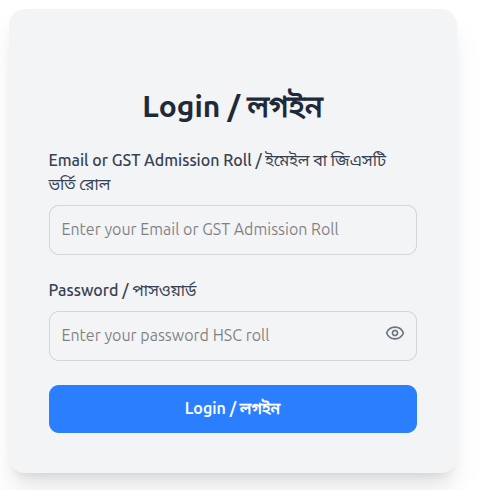
\includegraphics[width=0.6\textwidth]{chapters/chapter4/images/login.png}
    \caption{System Authentication (Login Page)}
    \label{fig:authentication_login}
\end{figure}


\section{Student Module Implementation}
After successful authentication, students are directed to their application portal. The primary task for a student is to complete the comprehensive admission form, providing accurate personal and academic information.

\subsection{Final Admission Form}
The admission form is designed to collect detailed geographical and identification data. To ensure data integrity, the system implements strict front-end validation for each input field.

\begin{figure}[htbp]
    \centering
    % Ensure your file is at this exact path: chapters/chapter4/images/form.png
    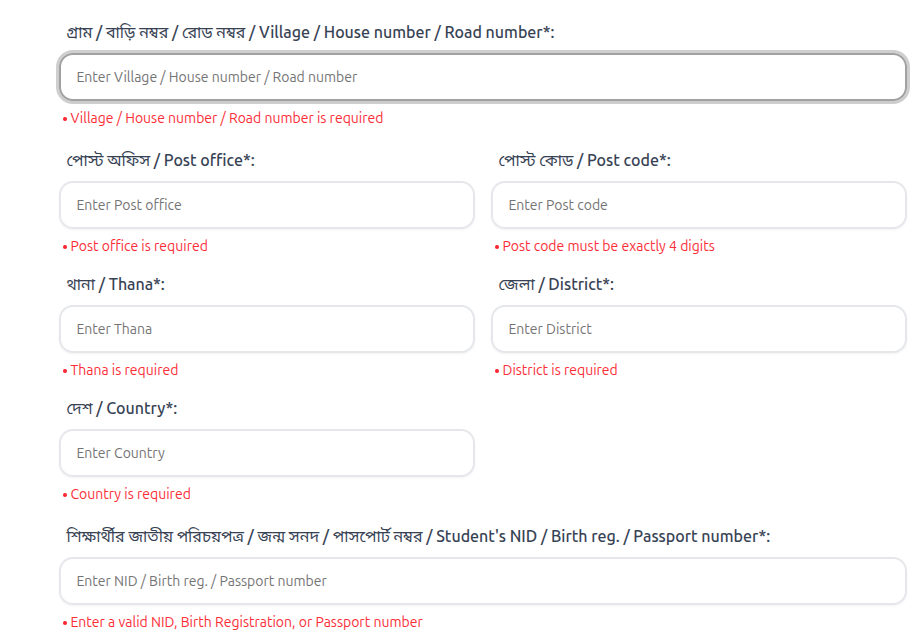
\includegraphics[width=0.85\textwidth]{chapters/chapter4/images/form.png}
    \caption{Student Admission Form with Validation}
    \label{fig:student_form}
\end{figure}

As shown in Figure \ref{fig:student_form}, the form focuses on the following components:

\begin{itemize}
    \item \textbf{Address Details:} The form requires the student's \textit{Village/House number}, \textit{Post Office}, \textit{Thana}, \textit{District}, and \textit{Country}. Each field is marked with an asterisk (*), indicating it is mandatory.
    \item \textbf{Postal Code Validation:} A specific validation rule is applied to the \textbf{Post Code} field, requiring exactly 4 digits, which prevents incorrect data entry.
    \item \textbf{Identification Information:} The system provides a flexible identification section where students must enter either their \textbf{NID}, \textbf{Birth Registration}, or \textbf{Passport number}.
    \item \textbf{Real-time Error Handling:} As illustrated in the figure, the system uses reactive validation. If a user leaves a field empty or enters invalid data (e.g., an incomplete post code), a red error message appears immediately below the input field to guide the user.
    \item \textbf{Bilingual Interface:} Continuing the design philosophy, all labels are provided in both Bengali and English to ensure clarity for all applicants.
\end{itemize}

This structured approach ensures that the database receives clean, formatted data, which simplifies the subsequent verification process by the Dean and Registrar offices.


\subsection{Application Summary and PDF Download}
After completing the necessary steps of the admission form, the student reaches the final stage where they can review their application summary and export the data for official use.

\begin{figure}[htbp]
    \centering
    
\includegraphics[width=0.8\textwidth]{chapters/chapter4/images/download.png}
    \caption{Final Application Submission and Download Interface}
    \label{fig:download_pdf_section}
\end{figure}

The features of this section, as shown in Figure \ref{fig:download_pdf_section}, are described below:

\begin{itemize}
    \item \textbf{Review Mechanism:} The \textit{Previous} button allows students to navigate back and double-check their provided information before final submission. This ensures that no incorrect data is sent to the university database.
    \item \textbf{Instant PDF Generation:} The system is integrated with a PDF generation library that converts the student's input fields into a formal document format. By clicking the \textbf{Download PDF} button, the user can instantly save a copy of their admission form.
    \item \textbf{Visual Feedback:} The button utilizes a distinct gradient color and a download icon to provide clear visual feedback, indicating that this is the primary action of the page.
    \item \textbf{Official Requirement:} This downloaded PDF acts as an acknowledgment slip, which contains a unique identifier for the student. It is mandatory for students to bring a printed copy of this document during the physical verification at the Dean's office.
\end{itemize}
\subsection{Submission Confirmation and Complaint Management}
Once a student successfully submits their application form, the system displays a confirmation message and provides options for subsequent necessary actions. This interface ensures the applicants that their data has been securely stored in the database.

\begin{figure}[htbp]
    \centering
    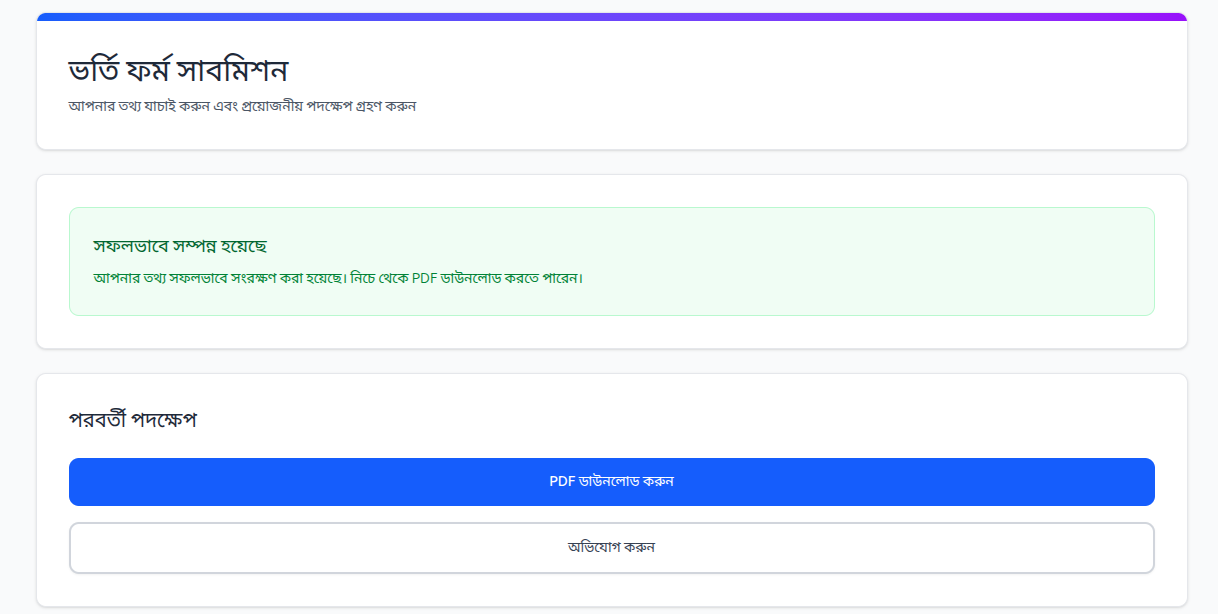
\includegraphics[width=0.85\textwidth]{chapters/chapter4/images/complain.png}
    \caption{Form Submission Confirmation and Complaint Interface}
    \label{fig:submission_status}
\end{figure}

As illustrated in Figure \ref{fig:submission_status}, the submission status page includes several key functional elements:

\begin{itemize}
    \item \textbf{Success Notification:} A green alert box is utilized to inform the student that their information has been successfully saved. This enhances the user experience and maintains system transparency.
    \item \textbf{PDF Generation and Download:} Students can download their completed application form in PDF format for future reference. This is a core component of the system's automated report generation module.
    \item \textbf{Complaint Management:} If a student notices any discrepancy in their data or encounters issues after submission, they can directly file a report through this integrated module.
    \item \textbf{Action Buttons:} The interface features clear and actionable buttons (e.g., "Download PDF" and "Complain"), which guide the user through the next steps without ambiguity.
\end{itemize}

Through this feature, system reliability is increased, and students are provided with immediate feedback and support options.


\section{Admin Module: Data and Resource Management}
The Admin module serves as the primary gateway for preparing the system for a new admission session.

\subsection{Bulk Data Import and External Storage Integration}
The administrator can populate the database by uploading Excel or SQL files containing GST admission results. To ensure data safety, a Google Drive integration is also provided.

\begin{figure}[H]
    \centering
    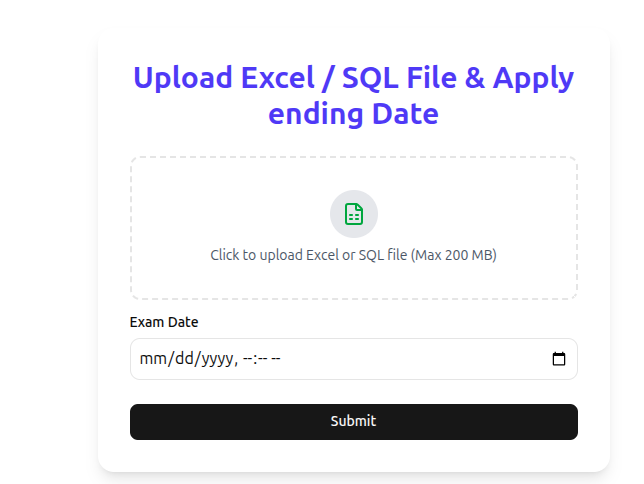
\includegraphics[width=0.75\textwidth]{chapters/chapter4/images/excelupload.png}
    \caption{Excel/SQL File Upload and Application Deadline Interface}
    \label{fig:excel_upload}
\end{figure}

\begin{itemize}
    \item \textbf{Data Ingestion:} The system parses the uploaded file and updates the applicant records. The interface also allows setting an "Exam Date" as a deadline.
    \item \textbf{Cloud Backup:} Using the interface shown in \textit{uploadDrive.png} (if applicable), the admin can sync local data with Google Drive for disaster recovery.
\end{itemize}

\subsection{Examination Announcement}
The admin defines the specific admission unit and the corresponding examination date to notify the applicants.

\begin{figure}[H]
    \centering
    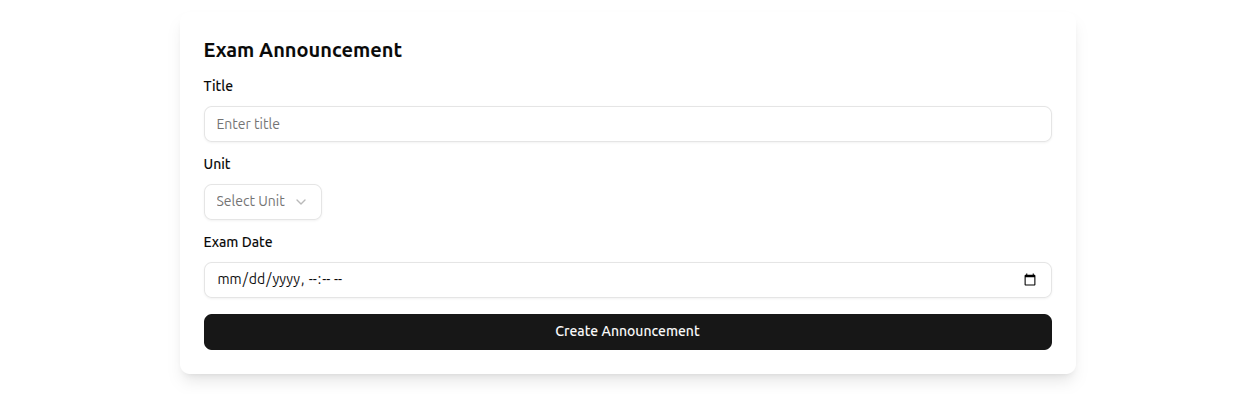
\includegraphics[width=0.75\textwidth]{chapters/chapter4/images/examAnoucement.png}
    \caption{Exam Announcement Configuration Interface}
    \label{fig:exam_announcement}
\end{figure}
\section{Admin Module: User Control and Security}
Security is managed through a comprehensive user administration panel that controls access for university officials.

\subsection{Role-Based Credential Generation}
The Admin can create specific accounts for Deans, Registrars, and Medical Officers using a dedicated credential creation form.

\begin{figure}[H]
    \centering
    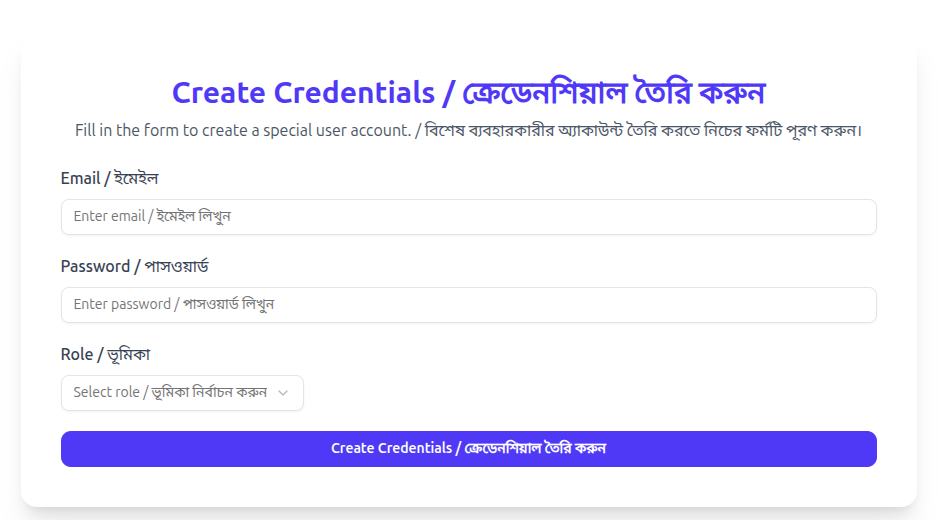
\includegraphics[width=0.75\textwidth]{chapters/chapter4/images/credentail.png}
    \caption{User Credential Creation Interface}
    \label{fig:create_credentials}
\end{figure}

\subsection{System User Monitoring}
A centralized dashboard allows the Admin to monitor all registered officials, their roles, and their account status.

\begin{figure}[H]
    \centering
    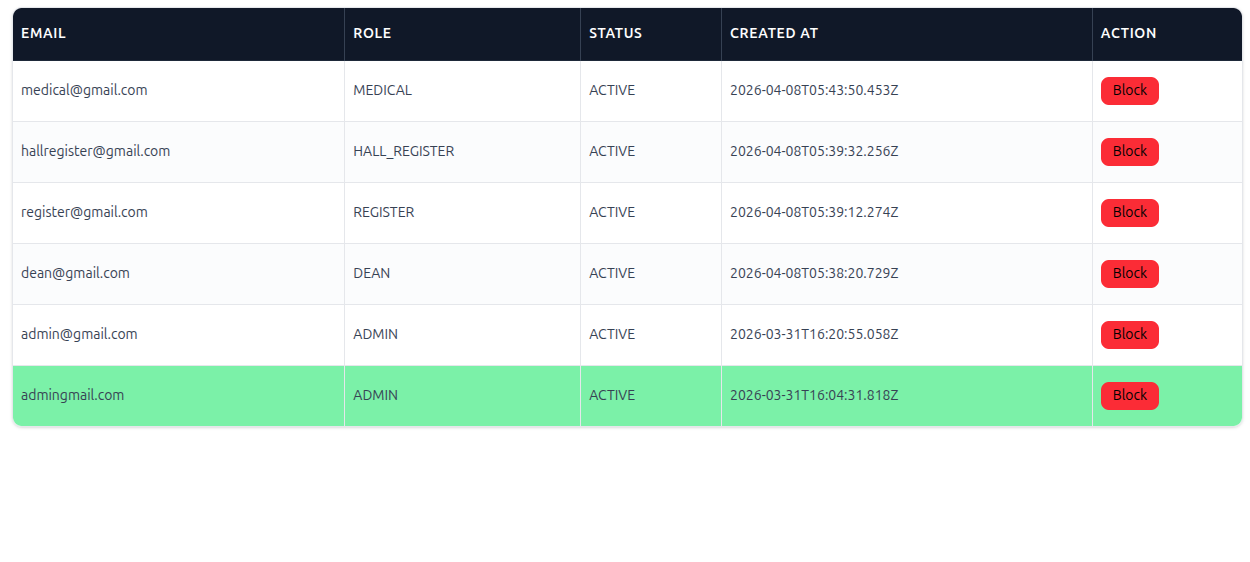
\includegraphics[width=0.9\textwidth]{chapters/chapter4/images/userManagement.png}
    \caption{Administrative User Management Dashboard}
    \label{fig:user_management}
\end{figure}

\begin{itemize}
    \item \textbf{Status Control:} Admins can "Block" or "Unblock" accounts instantly to prevent unauthorized access.
    \item \textbf{Role Identification:} The interface clearly labels the role (e.g., DEAN, REGISTER) and the timestamp of account creation.
\end{itemize}
\section{Admin Module: Complaint Resolution System}
To address student grievances, the Admin panel provides a real-time tracking system for complaints submitted through the student portal.

\subsection{Reviewing Pending Complaints}
All student issues are listed in a simplified queue, allowing administrators to address them systematically.

\begin{figure}[H]
    \centering
    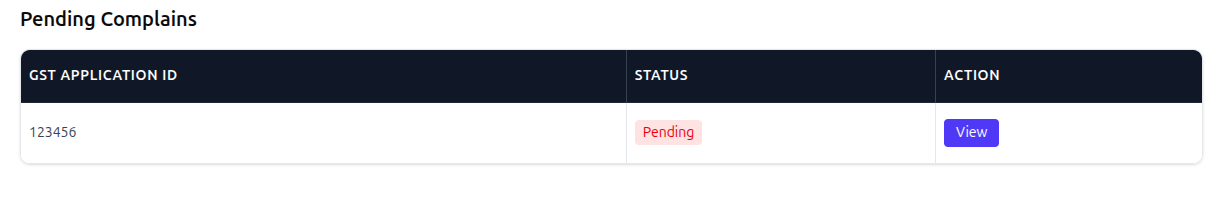
\includegraphics[width=0.85\textwidth]{chapters/chapter4/images/checkcomplain.png}
    \caption{Pending Complaint Tracking Interface}
    \label{fig:check_complain}
\end{figure}

The complaint handling workflow involves:
\begin{itemize}
    \item \textbf{Application ID Mapping:} Every complaint is mapped to a GST Application ID for cross-verifying academic records.
    \item \textbf{Detailed Action:} By clicking the "View" button, the admin can read the full text of the complaint and take necessary corrective measures.
\end{itemize}


% --- Dean Module (Divided) ---
\section{Dean Module: Applicant Verification}
The Dean's primary responsibility is to oversee the departmental applicant lists and verify the academic eligibility of the candidates.

\subsection{Departmental Applicant Queue}
The portal provides a real-time data table displaying students assigned to various departments under the faculty.

\begin{figure}[H]
    \centering
    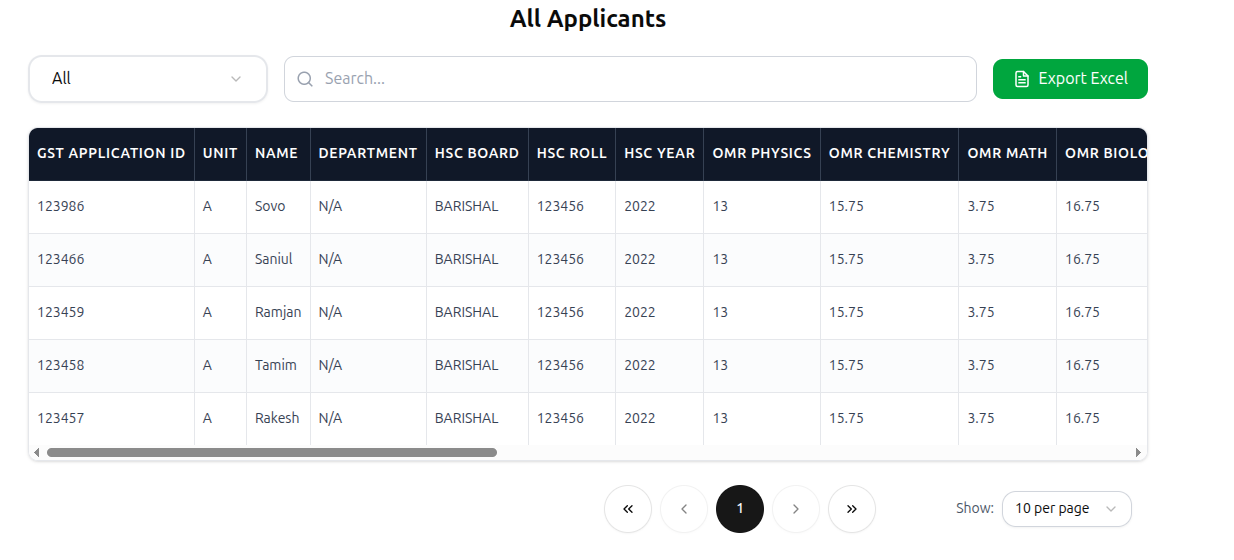
\includegraphics[width=0.9\textwidth]{chapters/chapter4/images/applicantList.png}
    \caption{Dean's Portal: Integrated Applicant List}
    \label{fig:dean_applicant_list}
\end{figure}

\subsection{Detailed Information Table}
To facilitate precise verification, a detailed list table is implemented that shows specific student attributes.

\begin{figure}[H]
    \centering
    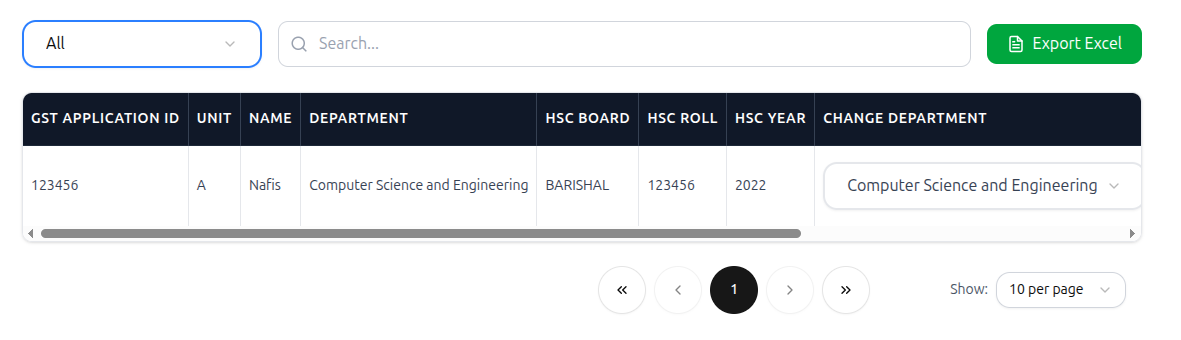
\includegraphics[width=0.9\textwidth]{chapters/chapter4/images/listTable.png}
    \caption{Dean's Detailed Data Verification Table}
    \label{fig:dean_list_table}
\end{figure}

The Dean uses this interface to cross-check GST scores and departmental requirements before moving to the approval stage.
\section{Dean Module: Student Status Management}

\noindent The Dean Module is for managing the status of students. The Dean has the power to approve a student for a department or cancel their application if there are problems with their records.

\setlength{\fboxsep}{6pt}
\setlength{\fboxrule}{1pt}
\begin{figure}[H]
    \centering
   \fbox{ 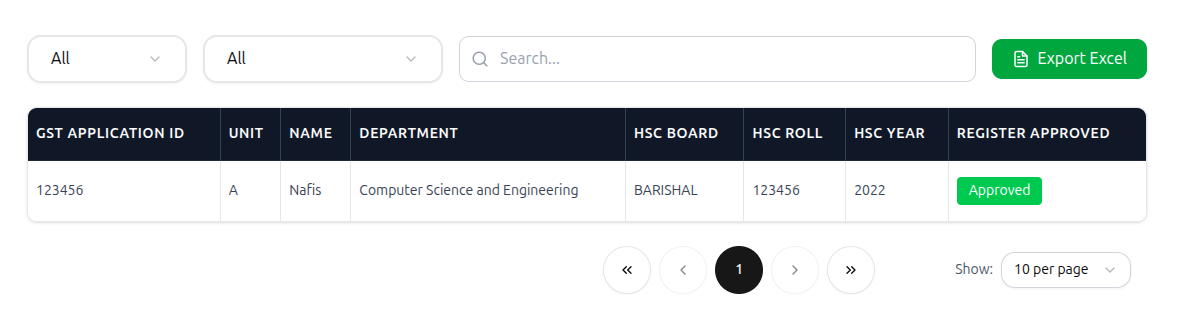
\includegraphics[width=0.8\textwidth]{chapters/chapter4/images/approvedList.png}}
    \caption{Dean’s Portal: Admission Approval and Cancellation Interface}
    \label{fig:dean_status_manage}
\end{figure}

\noindent The Dean can do these things:
\begin{itemize}
    \item {Approve Admission:} If a student's grades and documents are okay, the Dean can click the "Approve" button to send the student to the next step.
    \item {Cancel Admission:} If a student's information is fake or they do not meet the requirements of the department, the Dean can cancel their admission status.
\end{itemize}

\noindent The Dean Module is part of the Student Status Management system. The Dean uses the Deans Portal to make decisions about student admissions. The Dean’s decisions are final and affect the students’ status in the system. The Dean can cancel a student’s admission at any time.
% \section{Dean Module: Data Redundancy and Sync}
To ensure the security of academic records, the Dean's module is equipped with an automated data synchronization feature.

\subsection{Google Drive Integration}
The system allows the Dean to sync the verified applicant lists directly to a faculty-specific Google Drive account.

\begin{figure}[H]
    \centering
    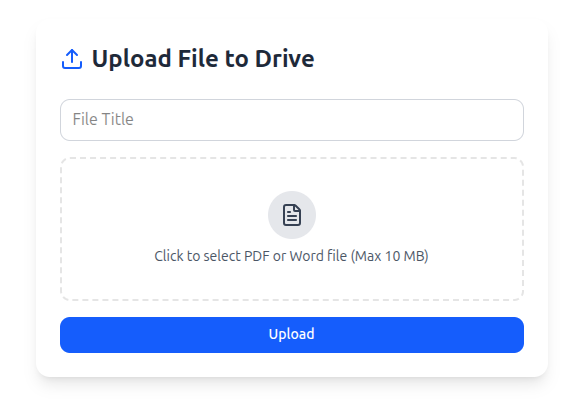
\includegraphics[width=0.7\textwidth]{chapters/chapter4/images/uploadDrive.png}
    \caption{Faculty Data Synchronization with Cloud Storage}
    \label{fig:dean_drive}
\end{figure}

This integration serves as a disaster recovery measure, ensuring that the Dean's office maintains a permanent record of all admitted students even in the event of local server issues.

% --- Registrar Module (Divided) ---
\section{Registrar Module: Centralized Data Validation}
The Registrar office holds the authority for the final validation of applicant data before the admission is officially confirmed. 

\subsection{Master Applicant Queue}
The Registrar monitors the global applicant list to oversee the progress of the admission session across all faculties.

\begin{figure}[H]
    \centering
    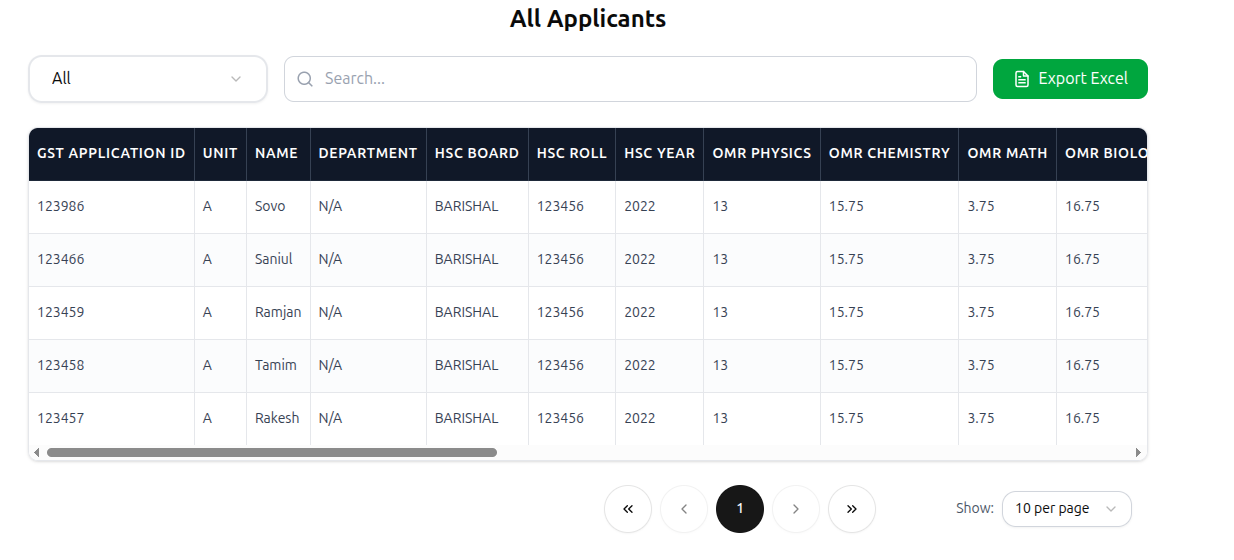
\includegraphics[width=0.9\textwidth]{chapters/chapter4/images/applicantList.png}
    \caption{Registrar's Master Applicant Data Interface}
    \label{fig:registrar_master_list}
\end{figure}

\subsection{Detailed Verification Matrix}
Using a more granular data table, the Registrar office cross-checks the physical document submission status with the digital records.

\begin{figure}[H]
    \centering
    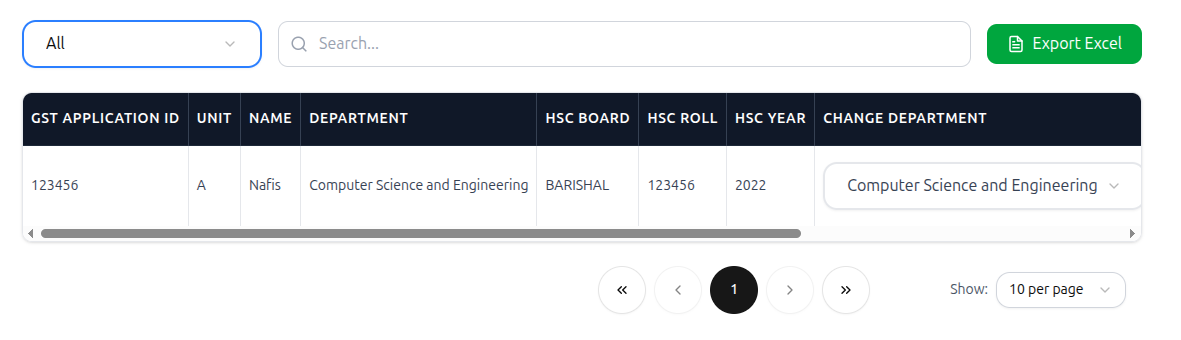
\includegraphics[width=0.9\textwidth]{chapters/chapter4/images/listTable.png}
    \caption{Registrar's Detailed Validation Table}
    \label{fig:registrar_table_view}
\end{figure}

This dual-layer verification ensures that only students with legitimate academic credentials and fee payments are processed for the final step.
\section{Registrar Module: Data Archiving and Redundancy}
As the primary record-keeper of the university, the Registrar's module emphasizes permanent data storage and cloud synchronization.

\subsection{Automated Cloud Backup}
To prevent data loss and ensure long-term accessibility, the system integrates a direct upload feature to the university's central Google Drive.

\begin{figure}[H]
    \centering
    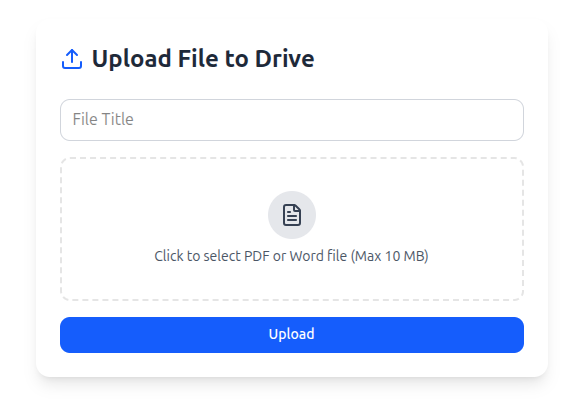
\includegraphics[width=0.7\textwidth]{chapters/chapter4/images/uploadDrive.png}
    \caption{Registrar's Archival System (Google Drive Sync)}
    \label{fig:registrar_archive}
\end{figure}

Through this interface, the Registrar can archive the entire session's data, providing a robust disaster recovery plan for the admission system.
\section{Registrar Module: Final Authorization}
The Registrar performs the final audit. This interface allows the Registrar to finalize the admission or reject it if any legal or official requirement is missing.
\setlength{\fboxsep}{6pt}
\setlength{\fboxrule}{1pt}
\begin{figure}[H]
    \centering
   \fbox{ 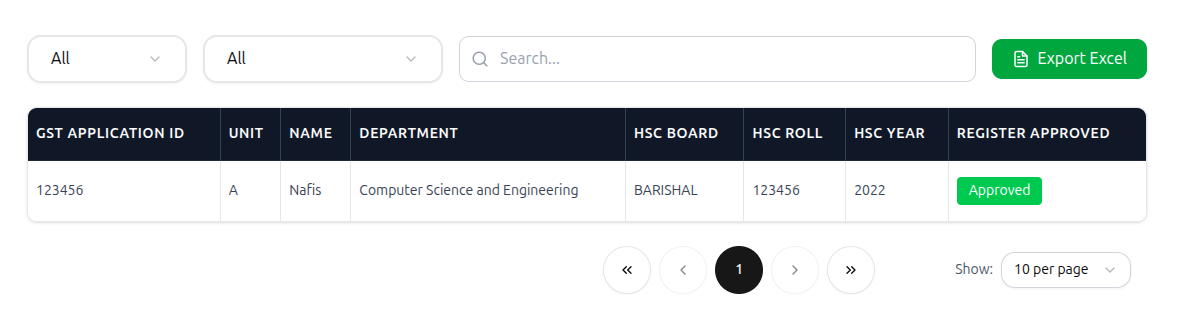
\includegraphics[width=0.8\textwidth]{chapters/chapter4/images/approvedList.png}}
    \caption{Registrar's Final Admission Authorization Dashboard}
    \label{fig:registrar_final_action}
\end{figure}

Through this dashboard, the Registrar ensures:
\begin{itemize}
    \item {Final Confirmation:} Authorized students are officially enrolled in the university database.
    \item {Admission Rejection:} The Registrar can cancel or revert an admission if the payment or official verification fails at the last moment.
\end{itemize}

% --- Hall Registrar Module (Divided) ---
\section{Hall Registrar: Residential Clearance}
The Hall Registrar manages the residential status. Only students with an "Approved" hall status are allowed to reside in the university halls.

\begin{figure}[H]
    \centering
    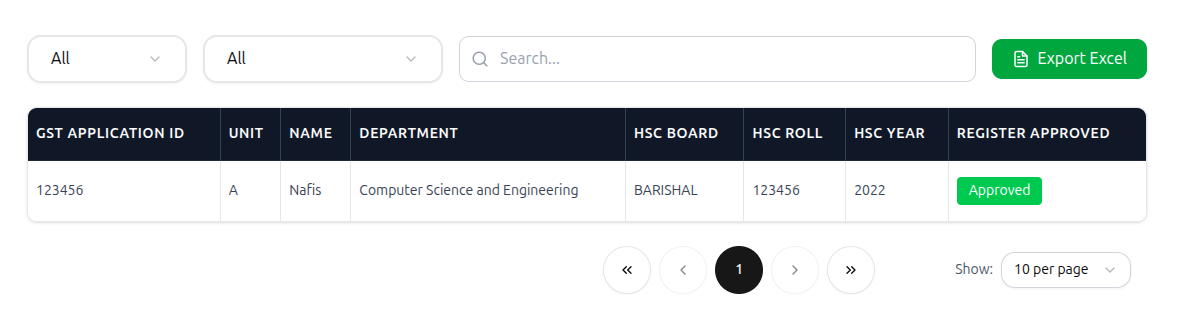
\includegraphics[width=0.85\textwidth]{chapters/chapter4/images/approvedList.png}
    \caption{Hall Allocation Approval and Cancellation View}
    \label{fig:hall_status_manage}
\end{figure}

\begin{itemize}
    \item \textbf{Seat Approval:} Assigning a hall name and room to the student.
    \item \textbf{Allocation Cancellation:} Removing a student from the hall list if they choose to stay off-campus or provide incorrect information.
\end{itemize}
\section{Hall Registrar Module: Resident Data Verification}
To ensure accurate record-keeping, the Hall Registrar utilizes a specialized queue to manage applicants who have applied for residential facilities.

\subsection{Hall Applicant Queue}
The interface displays a list of students who have cleared the academic and administrative stages and are now waiting for residential allocation.

\begin{figure}[H]
    \centering
    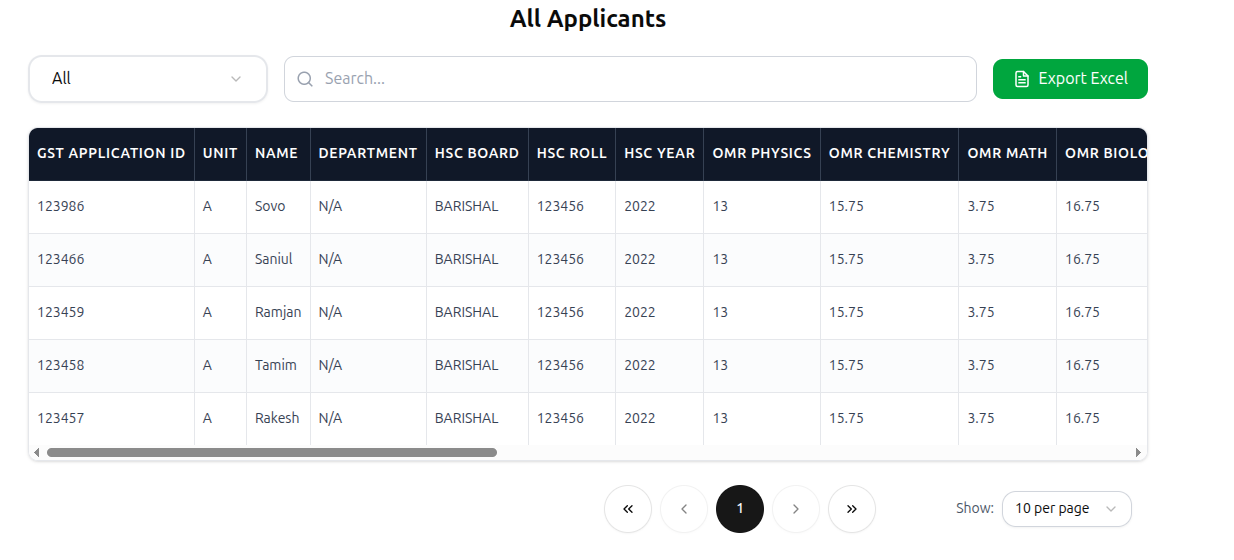
\includegraphics[width=0.9\textwidth]{chapters/chapter4/images/applicantList.png}
    \caption{Hall Resident Applicant Queue}
    \label{fig:hall_applicant_queue}
\end{figure}

\subsection{Detailed Resident Attributes}
The Hall Registrar can view specific student data, such as permanent address and gender, which are crucial factors in hall assignment.

\begin{figure}[H]
    \centering
    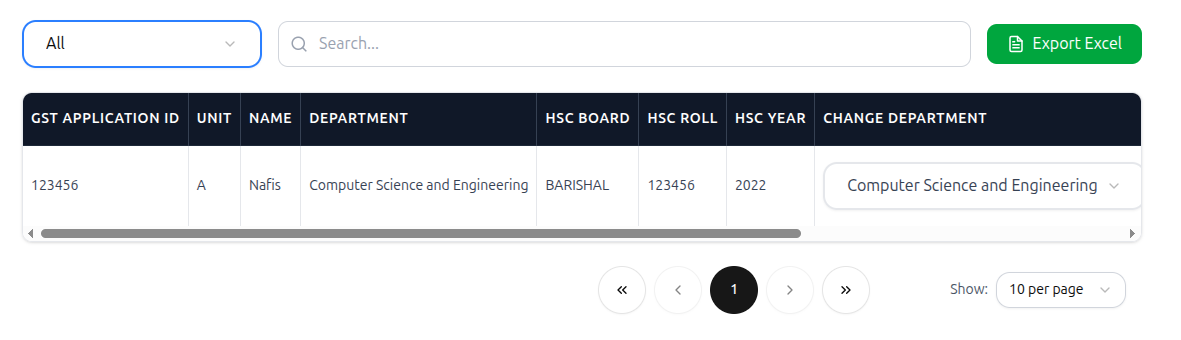
\includegraphics[width=0.9\textwidth]{chapters/chapter4/images/listTable.png}
    \caption{Detailed Resident Information Matrix}
    \label{fig:hall_resident_table}
\end{figure}
\section{Hall Registrar Module: Data Redundancy}
Due to the sensitivity of residential records, the Hall Registrar module includes a dedicated synchronization mechanism to preserve allocation data.

\subsection{Cloud Synchronization for Hall Records}
The Hall Registrar can sync the final residential allotment lists to a secure cloud platform, ensuring that hall offices have access to student data for room distribution.

\begin{figure}[H]
    \centering
    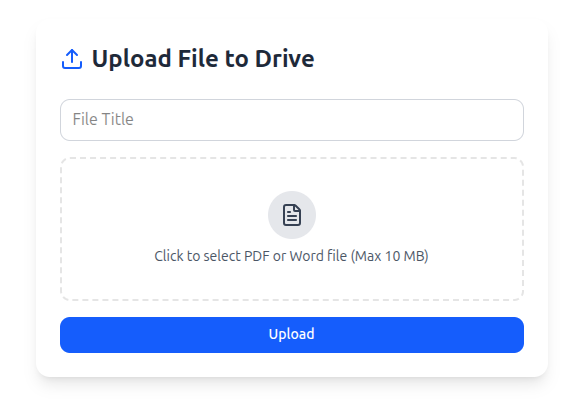
\includegraphics[width=0.7\textwidth]{chapters/chapter4/images/uploadDrive.png}
    \caption{Hall Office Data Sync and Backup}
    \label{fig:hall_drive_sync}
\end{figure}

This feature ensures data integrity and provides an offline reference for hall administration personnel.


% --- Medical Officer Module (Divided) ---
\section{Hall Registrar: Residential Clearance}
The Hall Registrar manages the residential status. Only students with an "Approved" hall status are allowed to reside in the university halls.


\setlength{\fboxsep}{6pt}
\setlength{\fboxrule}{1pt}
\begin{figure}[H]
    \centering
   \fbox{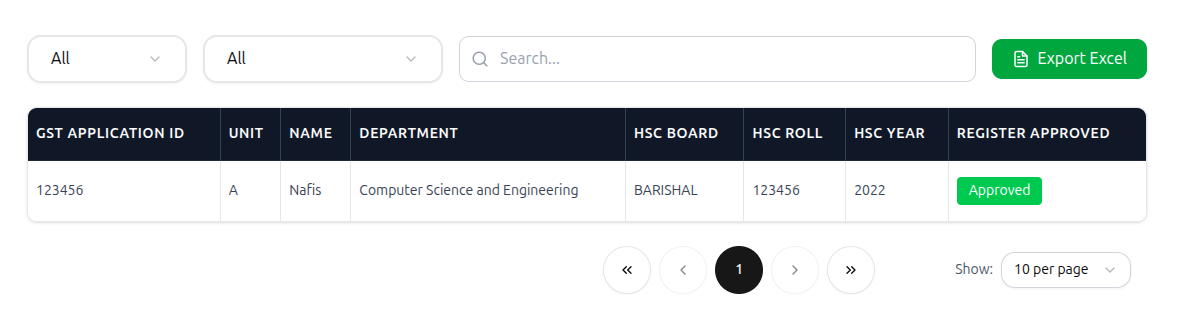
\includegraphics[width=0.8\textwidth]{chapters/chapter4/images/approvedList.png}}
    \caption{Hall Allocation Approval and Cancellation View}
    \label{fig:hall_status_manage}
\end{figure}

\begin{itemize}
    \item {Seat Approval:} Assigning a hall name and room to the student.
    \item {Allocation Cancellation:} Removing a student from the hall list if they choose to stay off-campus or provide incorrect information.
\end{itemize}
\section{Medical Officer Module: Applicant Health Data}
This section allows the Medical Officer to access the list of applicants who are awaiting medical checkups or record verification.

\subsection{Medical Verification Queue}
The portal displays a prioritized list of students who have completed their initial academic formalities and are now eligible for medical screening.

\begin{figure}[H]
    \centering
    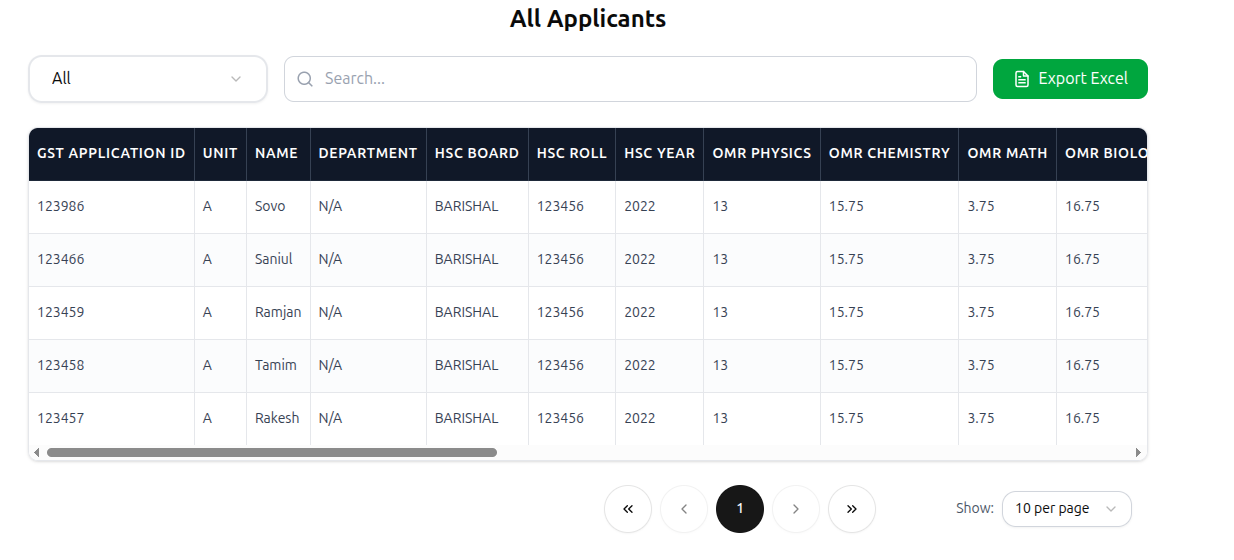
\includegraphics[width=0.9\textwidth]{chapters/chapter4/images/applicantList.png}
    \caption{Medical Officer's Applicant Screening Queue}
    \label{fig:medical_queue}
\end{figure}

\subsection{Detailed Medical Record Matrix}
A specialized table is used to view detailed student attributes, helping the medical staff to identify and document any specific health conditions.

\begin{figure}[H]
    \centering
    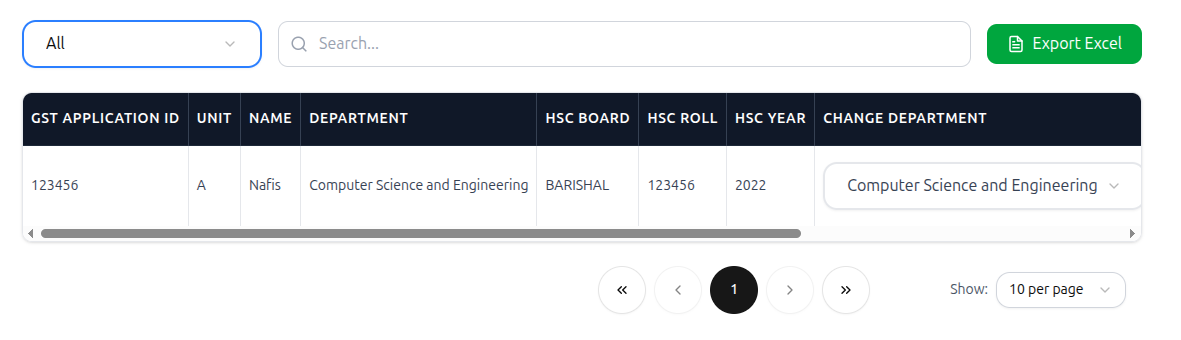
\includegraphics[width=0.9\textwidth]{chapters/chapter4/images/listTable.png}
    \caption{Detailed Health Record and Information Matrix}
    \label{fig:medical_record_table}
\end{figure}
% \section{Medical Officer Module: Data Synchronization}
To ensure the long-term safety of student health records, a cloud synchronization feature is integrated into the Medical Module.

\subsection{Cloud Backup for Health Records}
The Medical Officer can sync all health-related data and clearance reports to the university's central Google Drive for future medical history tracking.

\begin{figure}[H]
    \centering
    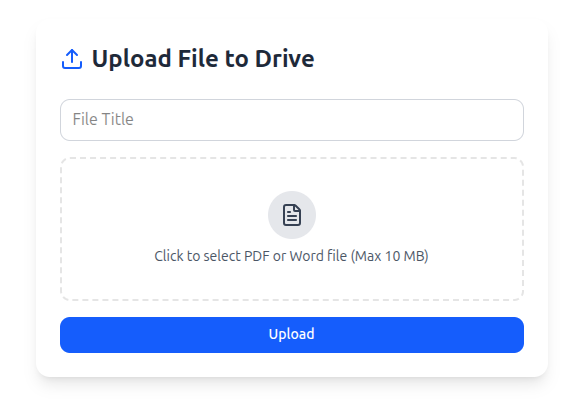
\includegraphics[width=0.7\textwidth]{chapters/chapter4/images/uploadDrive.png}
    \caption{Medical Data Archiving and Drive Integration}
    \label{fig:medical_drive_sync}
\end{figure}

This integration ensures that the university medical center maintains a persistent and secure digital record of all admitted students.
\chapter{Testing and Quality Assurance}

\setlength{\parindent}{0pt} % পুরো চ্যাপ্টারের জন্য ইন্ডেন্ট বন্ধ করা হলো

The Digital Admission Procedure Management for Post-GST Candidates needs to be tested well. This is an important part of making sure the system works correctly before we use it for the 2026 admission session. We want to make sure the Digital Admission Procedure Management for Post-GST Candidates is reliable, secure and correct.

\medskip
This part of the book explains how we tested the Undergraduate Final Admission System in many different ways from automatic tests to manual checks.

\section{Automated White Box Testing with Vitest}

We used Vitest to test the Undergraduate Final Admission System because it is built on the Next.js framework. Vitest helps us test the parts of the Digital Admission Procedure Management for Post-GST Candidates like the functions and components to make sure they work correctly.

\subsection{Component Rendering Tests}
We used Vitest and React Testing Library to test if the main parts of the user interface work properly. We checked to see if the main page navigation bar and admission form show up without any problems. The tests showed that the title of the Undergraduate Final Admission System and the important buttons are in the right place.

\subsection{Utility Function Testing}
We tested the functions that handle sensitive data like dates and scores. We tested a function that changes dates from the database into a format that's easy to read, like ``DD-MM-YYYY''. We also tested the functions that calculate scores to make sure they are correct.

\section{Backend API Testing with Postman}
We used Postman to test the backend of the Undergraduate Final Admission System, which was built with Node.js and Prisma. We sent kinds of requests to the backend to make sure it works correctly. We checked to see if the backend returns the information like a list of applicants with their scores and positions.

\section{Manual Functional Testing}
We did tests to make sure the Digital Admission Procedure Management for Post-GST Candidates works well from a users point of view. We tested the admission form to make sure it works correctly. We tried submitting the form without filling in all the required fields. We got an error message.

\subsection{Form Validation Testing}
We tested all the fields in the admission form to make sure they work correctly. We tried putting in the kind of information like letters in a field that only allows numbers.

\subsection{Role-Based Access Control (RBAC) Test}
We tested to make sure that different users can only access the parts of the Undergraduate Final Admission System that they are allowed to. We tried to access a part of the system that's only, for administrators and we were redirected to the login page.

\section{Summary of Test Results}
All the tests we did on the Undergraduate Final Admission System passed, which means it is working correctly. The table below shows the results of the tests.

\vspace{0.5cm}

\begin{table}[h]
    \centering
    \renewcommand{\arraystretch}{1.5}
    \begin{tabular}{|l|l|c|}
        \hline
        \textbf{Test Category} & \textbf{Testing Tool} & \textbf{Status} \\ \hline
        White Box Testing & Vitest & Passed \\ \hline
        API Testing & Postman & Passed \\ \hline
        Functional Testing & Manual & Passed \\ \hline
        Validation & Manual & Passed \\ \hline
        RBAC & Manual & Passed \\ \hline
    \end{tabular}
    \caption{Summary of Testing Results for JUST-DAPM-PGC}
    \label{tab:test_summary}
\end{table}
\chapter{Deployment and Conclusion}

The final phase of the software development life cycle is the deployment and delivery of the system to the production environment. This chapter discusses the deployment strategy used for the JUST Undergraduate Final Admission System (JUST-UFAS) and the future prospects of the project.

\section{Deployment Process}
Deploying a modern web application built with Next.js and Node.js involves a structured workflow to ensure stability and performance. The deployment process for JUST-UFAS followed these essential steps:

\begin{itemize}
    \item \textbf{Production Build:} The application code was optimized and compiled into a production-ready build to ensure fast loading times and efficient resource management.
    \item \textbf{Environment Configuration:} Essential environment variables, such as PostgreSQL database connection strings and Prisma client settings, were configured on the production server.
    \item \textbf{Server Setup:} The application is hosted on the university's official infrastructure. Due to existing resource allocations, the system is currently deployed on a specific port.
    \item \textbf{Maintenance and Monitoring:} The system is actively maintained by the \textbf{Technical Committee of Undergraduate Admission} at Jashore University of Science and Technology.
\end{itemize}

\section{Deployment Status and URL}
The system is currently live and accessible for the final admission process. 

\begin{itemize}
    \item \textbf{Current Hosting:} The project is running on the university's existing domain using port 3000 as a cost-effective hosting solution.
\end{itemize}

\section{Conclusion}
The "JUST Undergraduate Final Admission System" offers a significant improvement over manual admission processes. By automating the workflow, the system has achieved:
\begin{itemize}
    \item \textbf{Efficiency:} Faster data processing and reduced manual labor.
    \item \textbf{Accuracy:} Minimized human errors in student data handling and merit list verification.
    \item \textbf{Cost-Effectiveness:} Reduced need for extra manpower, leading to operational cost savings for the university.
\end{itemize}

\section{Future Work}
While the current system fulfills all primary requirements, future updates could include:
\begin{itemize}
    \item \textbf{Automated Migration:} Implementing a full auto-migration system for students across different departments.
    \item \textbf{Payment Gateway Integration:} Integrating local mobile banking (bKash, Nagad) for seamless admission fee collection.
    \item \textbf{Mobile Application:} Developing a dedicated mobile app for students to track their admission status in real-time.
\end{itemize}

Through this project, Jashore University of Science and Technology has taken a step forward in digitizing its administrative infrastructure, ensuring a smoother experience for future students.

\chapter{Conclusion}


\noindent The deployment of the Digital Admission Procedure Management system marks the successful transition of the application from development to a real-world operational environment. Through proper configuration of the backend and frontend components, the system has been effectively hosted on the university infrastructure, ensuring accessibility for end-users.

\vspace{0.3cm}

\noindent This deployment demonstrates the practicality and reliability of the system in managing the admission process in a more efficient and automated manner. It reduces manual workload, improves data handling accuracy, and ensures smoother communication between applicants and the administrative office.

\vspace{0.3cm}

\noindent Although the system is currently fully functional, there is still room for future enhancements such as mobile application support, improved scalability, and integration of advanced technologies like artificial intelligence. These improvements can further increase usability and performance.

\vspace{0.3cm}

\noindent Overall, the deployment phase confirms that the Digital Admission Procedure Management system is a successful step toward digitalizing the admission process at Jashore University of Science and Technology.

\vspace{0.3cm}

\noindent
Another key aspect brought out by the implementation process is the role of cooperation between the development team and the administrative body of the institution. It ensures that the software application fulfills all institutional needs and reflects the actual admission process.On another note, the software application has been created to be scalable and thus capable of being expanded without any need to redesign.

\section*{References}

\begin{itemize}

\item Next.js Documentation. \url{https://nextjs.org/docs} (Accessed: Sep 2025)

\item React Documentation. \url{https://react.dev} (Accessed: Oct 2025)

\item TypeScript Documentation. \url{https://www.typescriptlang.org/docs} (Accessed: Oct 2025)

\item JavaScript Guide - MDN. \url{https://developer.mozilla.org/en-US/docs/Web/JavaScript} (Accessed: Nov 2025)

\item Node.js Documentation. \url{https://nodejs.org/en/docs} (Accessed: Nov 2025)

\item Express.js Documentation. \url{https://expressjs.com} (Accessed: Nov 2025)

\item PostgreSQL Documentation. \url{https://www.postgresql.org/docs} (Accessed: Dec 2025)

\item Prisma ORM Documentation. \url{https://www.prisma.io/docs} (Accessed: Dec 2025)

\item Tailwind CSS Documentation. \url{https://tailwindcss.com/docs} (Accessed: Dec 2025)

\item W3Schools HTML Tutorial. \url{https://www.w3schools.com/html/} (Accessed: Jan 2026)

\item W3Schools CSS Tutorial. \url{https://www.w3schools.com/css/} (Accessed: Jan 2026)

\item W3Schools JavaScript Tutorial. \url{https://www.w3schools.com/js/} (Accessed: Jan 2026)

\item NPM Documentation. \url{https://docs.npmjs.com} (Accessed: Jan 2026)

\item Git Documentation. \url{https://git-scm.com/doc} (Accessed: Feb 2026)

\item GitHub Documentation. \url{https://docs.github.com} (Accessed: Feb 2026)

\item REST API Guide. \url{https://restfulapi.net} (Accessed: Feb 2026)

\item HTTP Overview - MDN. \url{https://developer.mozilla.org/en-US/docs/Web/HTTP} (Accessed: Feb 2026)

\item JSON Official Website. \url{https://www.json.org} (Accessed: Feb 2026)

\item JWT Introduction. \url{https://jwt.io} (Accessed: Mar 2026)

\item Axios Documentation. \url{https://axios-http.com} (Accessed: Mar 2026)

\item dotenv NPM Package. \url{https://www.npmjs.com/package/dotenv} (Accessed: Mar 2026)

\item CORS Guide - MDN. \url{https://developer.mozilla.org/en-US/docs/Web/HTTP/CORS} (Accessed: Mar 2026)

\item bcrypt Password Hashing Library. \url{https://www.npmjs.com/package/bcrypt} (Accessed: Mar 2026)

\item Zod Validation Library. \url{https://zod.dev} (Accessed: Mar 2026)

\item Prisma Migrate Guide. \url{https://www.prisma.io/docs/orm/prisma-migrate} (Accessed: Apr 2026)

\item Vercel Deployment Platform. \url{https://vercel.com/docs} (Accessed: Apr 2026)

\item Render Cloud Deployment. \url{https://render.com/docs} (Accessed: Apr 2026)

\item Swagger API Documentation. \url{https://swagger.io/docs} (Accessed: Apr 2026)

\item Axios HTTP Client Docs. \url{https://axios-http.com/docs/intro} (Accessed: Apr 2026)

\item Web Security Basics. \url{https://developer.mozilla.org/en-US/docs/Web/Security} (Accessed: Apr 2026)

\item Software Engineering Principles (Pressman Reference, 2025 Edition)

\item Clean Code Principles - Robert C. Martin (2019 Edition)

\end{itemize}

\end{document}